\documentclass[12pt,number,sort&compress,preprint]{elsarticle}

%======================================================================
\usepackage{todonotes}
\usepackage{graphicx}
\usepackage[binary-units]{siunitx}
\usepackage{gensymb}
\usepackage[version=3]{mhchem} % Formula subscripts using \ce{}, e.g., \ce{H2SO4}
\usepackage{booktabs,multicol} %better tables
\usepackage{subcaption} %subfigs
\usepackage{lmodern}
\usepackage[T1]{fontenc}
\usepackage{textcomp}

% shared equations in separate file
% https://yatb.giacomodrago.com/en/post/3/latex-loading-equations-from-an-external-file.html
\usepackage{catchfilebetweentags}

% external references https://tex.stackexchange.com/a/14365/56227
\usepackage{xr-hyper}

\usepackage{amsmath,eqparbox,xparse,mathtools}

% load common macros / commands
\usepackage{macros}

\usepackage[breaklinks=true, linkcolor=blue, citecolor=blue, colorlinks=true]{hyperref}
% load after hyperref
\usepackage[english,capitalise]{cleveref}


%%%%%%%%%%%%%%%%%%%%%%%%%%%%
%      Custom Commands     %
%%%%%%%%%%%%%%%%%%%%%%%%%%%%


\sisetup{group-separator={,},
	detect-all,
	binary-units,
	list-units = single,
	range-units = single,
	range-phrase = --,
	per-mode = symbol-or-fraction,
	separate-uncertainty = true,
	multi-part-units = single,
	list-final-separator = {, and }
	%    scientific-notation = fixed
}

\DeclareSIUnit\doubles{doubles}

% load external document after hyperref https://tex.stackexchange.com/a/281417/56227
\externaldocument[deriv-]{derivations}

%======================================================================
% Add your bibliography file here, replace template.bib
\bibliographystyle{elsarticle-num}

% set figure path
\graphicspath{{./figures/}}


\title{SIMD\slash SIMT-vectorized Sparse Chemical Kinetic Jacobian\slash Thermo-chemical Source-Term Evaluation}

\author[1]{Nicholas Curtis\corref{corr}}
\ead{nicholas.curtis@uconn.edu}
\author[1]{Chih-Jen Sung}

\address[1]{Department of Mechanical Engineering, University of Connecticut, Storrs, CT 06269, USA}
\cortext[corr]{Corresponding author}

\begin{document}

\begin{frontmatter}

%====================================================================
\begin{abstract} % not to exceed 200 words
A code generation platform for single-instruction, multiple-data (SIMD) and single-instruction, multiple thread (SIMT) vectorized thermo-chemical source-term and sparse\slash dense chemical kinetic Jacobian evaluation was developed and validated for a wide range of chemical kinetic models.

\todo[inline]{this}
\end{abstract}

% (Provide 2-4 keywords describing your research. Only abbreviations firmly
% established in the field may be used. These keywords will be used for
% sessioning/indexing purposes.)
\begin{keyword}
    Chemical Kinetics\sep SIMD\sep SIMT\sep Sparse\sep Jacobian
\end{keyword}

\end{frontmatter}

%====================================================================
\section{Introduction}
%

As the importance of detailed chemical kinetics for predictive reactive-flow simulations has become recognized~\cite{LU2009192}, the size and complexity of chemical kinetic models describing current and next-generation fuels relevant to transportation and power generation have increased greatly; e.g., a recent biodiesel model~\cite{WESTBROOK2011742} consists of \textasciitilde\num{3500} chemical species, and over \num{17000} reactions.
Moreover, the cost of evaluating the chemical source-terms scales linearly with the size of the model, while evaluation and factorization of the chemical kinetic Jacobian---if naively implemented---scale quadratically and cubically with the number of species in the model~\cite{LU2009192}.
These factors often make the use of detailed chemical kinetics prohibitive in practice; e.g., in a recent direct numerical simulation~\cite{Spafford:2010aa} utilizing a 22-species model, evaluation of reaction rates consumed around half of the total run time.
In addition, chemical kinetic Jacobian evaluation and factorization---utilized by most common implicit integration techniques to deal with numerical stiffness---is a bottleneck for even modestly-sized chemical models in realistic reactive flow simulations, necessitating use of other cost-reduction strategies~\cite{LU2009192}.

A host of techniques have been developed to lessen the computational demand of chemical kinetic calculations while maintaining fidelity, these fall broadly into a few categories: removal of unimportant species and reactions unimportant species and reactions~\cite{Lu:2006bb,Pepiot-Desjardins:2008,Hiremath:2010jw,Niemeyer:2010bt,Curtis:2015}, lumping of species with similar thermo-chemical properties~\cite{Lu:2007,Ahmed:2007fa,Pepiot:2008kq}, and time-scale methods that reduce chemical stiffness~\cite{Maas:1992ws,Lam:1994ws,Lu:2001ve,Gou:2010}.
The interested reader is referred to the recent review of Tur\'anyi and Tomlin~\cite{turanyi2016analysis} for a comprehensive overview.
In addition to the previously mentioned cost reduction methods, effort has gone into improving the integration algorithms and codes that evaluate the chemical kinetics~\cite{Gou:2010,SCHWER2002270,Niemeyer:2016aa,GAO2015287}.
In particular, a carefully derived analytical formulation of the Jacobian can greatly increase the sparsity of the matrix~\cite{SCHWER2002270} and drop the cost of Jacobian evaluation from scaling quadratically with the number of species in the model---for a naive finite-difference implementation---to a linear dependence~\cite{LU2009192}, while Jacobian factorization can be accelerated via sparse-matrix techniques~\cite{superlu99}.
Use of Single-Instruction, Multiple-Data (SIMD) and the related Single-Instruction, Multiple-Thread (SIMT) processors to accelerate chemical kinetic simulations has also been studied, e.g., as in~\cite{CurtisGPU:2017,Sewerin20151375,Shi:2012aa,Niemeyer:2016aa}.

SIMD and SIMT programming are two important vector-processing paradigms used increasingly in scientific computing.
Traditional multi-core parallelism is often used to increase central processing unit (CPU) performance, however as exponential growth in processing power---colloquially known as Moore's law---has slowed~\cite{khan2018science}, SIMD processors as well as SIMT processors, e.g., in the form of graphics processing units (GPUs), have gained recognition due to their increased floating operation throughput.
The parallel programming standard OpenCL~\cite{stone2010opencl} has further enabled adoption of vector-processing based codes in scientific computing by providing a common application program interface (API) for execution on heterogeneous systems, e.g., the CPU, GPU, or Intel's Many Integrated Core architecture (MIC), etc.
In this discussion, we will largely use OpenCL terminology to describe these processing paradigms, as it provides a convenient way to classify otherwise disparate processor type (e.g., CPUs and GPUs), however the concepts discussed are broadly applicable to SIMD\slash SIMT processing and not tied to OpenCL specifically.

\begin{figure}[htb]
  \centering
  \begin{subfigure}[t]{0.45\linewidth}
      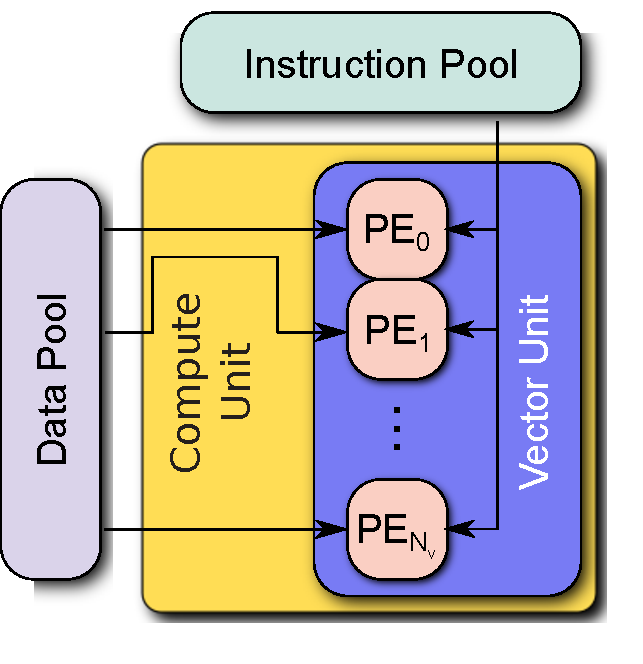
\includegraphics[width=\textwidth]{SIMD.pdf}
      \caption{Schematic of SIMD processing.  A single compute unit (e.g., a CPU core) contains a vector unit with $N_v$ processing elements, together called a vector-lane.  The vector unit executes a single instruction concurrently on multiple data.}
      \label{F:SIMD}
  \end{subfigure}
  \hfill
  \begin{subfigure}[t]{0.45\linewidth}
      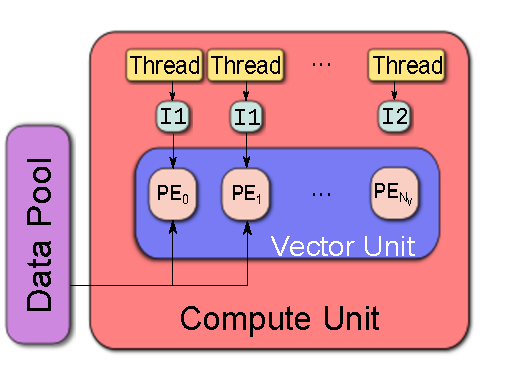
\includegraphics[width=\textwidth]{SIMT.pdf}
      \caption{Schematic of SIMT processing. A single compute unit (e.g., a GPU streaming multiprocessor) contains many processing elements and hosts many threads, each with an instruction to execute (I1, I2).  Threads with the same instruction execute concurrently on multiple data while the others must wait (leading to thread divergence).}
      \label{F:SIMT}
  \end{subfigure}
\end{figure}

A typical modern CPU has many compute units (i.e., cores), each with specialized vector processing units capable of running SIMD instructions (\cref{F:SIMD}).
A SIMD instruction utilizes the vector processor to execute the same floating point operation (e.g. multiplication, division, etc.) on a several different data concurrently; the number of concurrent operations possible is known as the vector-width\footnote{OpenCL allows for use of vector-widths different from the actual hardware vector-width via implicit conversion, and may provide some performance benefit as will be studied in Sec.~\ref{S:results}} and is typically around 2--4 double precision operations. 
Additionally, specialized hardware accelerators, e.g. Intel's Xeon Phi co-processor (MIC) have been developed that have tens of cores with very wide vector-widths (e.g. 4--8 double precision operations); these very wide vector-widths are also found on cutting-edge and forthcoming Intel CPUs; i.e., the Skylake Xeon and Cannon Lake architectures, respectively.

SIMT processing---the foundation of modern GPUs~\cite{lindholm2008nvidia}---is a related computing paradigm that hosts large numbers of threads on a single compute element (a streaming multiprocessor in NVIDIA terminology).
A group of threads---typically \num{32}, known as a warp on NVIDIA GPUs---execute the same SIMD instruction on multiple data concurrently (\cref{F:SIMT}).
If some threads must execute a different instruction---e.g., due to if\slash then branching or predication---they are forced to wait and execute later.
This phenomena, known as thread-divergence, is a key consideration for SIMT-processing and can cause serious performance degradation for complicated algorithms~\cite{CurtisGPU:2017}.

\subsection{Previous works and goals of this study}


Recognizing the need to accelerate Jacobian evaluation and factorization, a number of recent works have been published on analytical chemical kinetic Jacobian evaluation; although as will be discussed at the end of this section, this work offers several key improvements over past efforts.
The \texttt{TChem} software package~\cite{Safta:2011vn} was one of the first packages developed providing this functionality, but has several limitations including: incompatibilities with modern reaction types---i.e., pressure dependent Arrhenius (or P-Log) and Chebyshev reactions---and lack of thread-safety to enable parallel execution~\cite{Curtis2017:tchem}. 
Youssefi~\cite{Youssefi:2011tm} explored the importance of analytical Jacobian matrices for time-scale analysis techniques as well as their effect on computational efficiency in zero-dimensional homogeneous reactor simulations.
Bisetti~\cite{Bisetti:2012jw} developed an isothermal, isobaric analytical Jacobian code-generation utility; although incompatible with many combustion codes, a significant increase in Jacobian sparsity was exhibited.
Additionally, in the same work Bisetti provided a novel way to compute dense matrix-vector multiplications resulting from a change of system variables without need for storage of the full dense Jacobian.
Perini et al.~\cite{Perini:2012gy} developed an analytical Jacobian code for constant-volume combustion, with additional options to increase sparsity (at expect of strict correctness), and enable tabulation of temperature dependent properties; a \SI{80}{\percent} speedup over a finite-difference-based Jacobian was reported when used in a multidimensional reactive-flow simulation.
Dijkmans et al.~\cite{Dijkmans:2014bb} developed a GPU-based analytical Jacobian code with optional tabulation of temperature-dependent properties, and found speedups up to \SI{120}{$\times$} for zero-dimensional chemical kinetic integration with large chemical models (\textasciitilde\num{3000} species) with a Tesla C2075 GPU.
Niemeyer et al.~\cite{Niemeyer:2016aa} created and validated the open-source analytical chemical kinetic Jacobian code-generator, \texttt{pyJac}, supporting parallel execution on the CPU and SIMT execution on the GPU; a speedup of \SIrange{3}{7.5}{$\times$} over a finite-difference Jacobian was found on the CPU.
Gao et al.~\cite{GAO2015287} derived a sparse analytical Jacobian, but it was not validated outside the context of use with an implicit-integration technique; in addition the Jacobian was based on an over-constrained system, the effect on strict conservation of mass\slash energy was not studied.

A number of recent works have investigated the use of high-performance SIMT-devices to accelerate reactive-flow and chemical kinetics simulations.
Spafford et al.~\cite{Spafford:2010aa} investigated an implementation of an explicit direct numerical simulation code for compressible turbulent combustion on a Tesla C1060 GPU, and found an order of magnitude speedup in evaluation of species production rates as compared to a serial CPU implementation on an AMD-Opteron processor.
Shi et al.~\cite{Shi:2011aa} developed a code to evaluate species production rates and factorize the chemical kinetic Jacobian on a Tesla C2050 GPU, and found an order of magnitude speedup during integration of large chemical models when these operations were offloaded to the GPU as compared to the standard \texttt{CHEMKIN}~\cite{kee1989chemkin} and \texttt{LAPACK}~\cite{Anderson:1999aa} libraries on a quad-core Intel i7 930 CPU; it was not clear how\slash if the CPU code was parallelized.
Niemeyer et al.~\cite{Niemeyer:2011aa} implemented an explicit fourth-order Runge--Kutta integrator for non-stiff chemical kinetic integration on a Tesla C2075 GPU, and found a speedup of nearly two orders of magnitude when compared with a sequential CPU-code on an Intel Xeon X5650 CPU.
Shi et al.~\cite{Shi:2012aa} later extended their work to develop a stabilized-explicit solver on a Tesla C2050, paired with a traditional implicit integrator on quad-core Intel i7 930 which handled the stiffest computational cells; a \SIrange{11}{46}{$\times$} speedup was achieved over the base implicit CPU integrator during simulation of a three-dimensional premixed diesel engine simulation.
Le et al.~\cite{Le2013596} implemented two high-order shock-capturing reactive-flow codes on a Tesla C2070, and found a \numrange{30}{50}$\times$ speedup over a sequential CPU version of the same code on a Intel Xeon X5650.
Stone and Davis~\cite{Stone:2013aa} implemented the implicit VODE~\cite{Brown:1989vl} integrator on a Fermi M2050 GPU, achieving an order of magnitude speedup over the baseline CPU version on a single core of an AMD Opteron 6134 Magny-Cours.
Niemeyer and Sung~\cite{Niemeyer:2014aa} later developed a stabilized explicit second-order Runge--Kutta--Chebyshev algorithm on a Tesla C2075, demonstrating an order of magnitude speedup for a over a CPU implementation of VODE on a six-core Intel X5650 for moderately stiff chemical kinetics.
Sewerin and Rigopoulos~\cite{Sewerin20151375} implemented a three-stage\slash fifth-order implicit Runge--Kutta method~\cite{wanner1991solving} on both a high-end (NVIDIA Quadro 6000) and consumer-grade (NVIDIA Quadro 600) GPUs, as well as a standard CPU (two-core, four-thread Intel i5-520M) and a scientific workstation (eight-core, 16-thread Intel Xeon E5-2687W); the high-end GPU was at best \SI{1.8}{$\times$} slower than the workstation CPU (16 threads), while the consumer level GPU was at best \SI{5.5}{$\times$} slower than the corresponding standard CPU (four threads).
Yonkee and Sutherland~\cite{Yonkee2016} implemented GPU-accelerated evaluations of thermodynamic parameters, multicomponent transport properties and species production rates for solution of a partial differential equations (PDEs) on an Intel Xeon E5-2680 CPU and a Tesla K20 GPU.
In evaluation of the thermo-chemical properties, speedups between \SIrange{8}{13}{$\times$} were found (over a serial version of the same code) while running on 16 CPU cores, and \SIrange{20}{40}{$\times$} on the GPU; speedups of \textasciitilde\SI{9}{$\times$} and \textasciitilde\SI{25}{$\times$} were found in solution of a partially premixed methanol flame PDE on 16 CPU cores and the GPU respectively.
Curtis et al.~\cite{CurtisGPU:2017} implemented a fifth-order implicit Runge--Kutta method~\cite{wanner1991solving}, as well as two-fourth order exponential integration techniques~\cite{Hochbruck:1998,Hockbruck:2009} paired with an analytical Jacobian code~\cite{Niemeyer:2016aa} on a Tesla C2075; the implicit Runge--Kutta method was roughly equivalent to a standard implicit integrator~\cite{Hindmarsh:2005} running on 12--38 Intel Xeon E5-4640 v2 CPU cores for two smaller chemical models with an integration time step of \SI{e-6}{$\sec$}.

In contrast, SIMD-based chemical kinetics evaluation\slash integration have been far less studied.
Linford et al.~\cite{Linford:2011} implemented a three-stage, second-order Rosenbrock integrator for atmospheric chemical kinetics on the CPU, GPU and cell croadband engine (CBE)---a specially designed vector processor---and found speedups regularly exceeding~\SI{25}{$\times$} over a serial CPU implementation.
Kroshko and Spiteri~\cite{kroshko2013efficient} implemented a SIMD-vectorized third-order stiff Rosenbrock integrator for atmospheric chemistry on the CBE and found a speedup of \SI{1.89}{$\times$} (a parallel scaling efficiency of \SI{0.94}{$\percent$}) over a serial version of the same code.
Stone et al.,~\cite{stone2016} implemented a linearly-implicit fourth-order stiff Rosenbrock solver in the OpenCL for various platforms including CPUs, GPUs, and MICs.
SIMD-vectorization improved the integrator performance over an OpenMP baseline (which was vectorized by simple compiler hints (i.e., \texttt{\#pragmas}) by \SIrange{2.5}{2.8}{$\times$} on the CPU and \SIrange{4.7}{4.9}{$\times$} on the MIC, while the GPU performance was only \SIrange{1.4}{1.6}{$\times$} faster than the OpenMP baseline due to thread-divergence concerns.

This work will build upon our previous analytical chemical kinetic Jacobian code, \texttt{pyJac}~\cite{Niemeyer:2016aa}, in order to:
\begin{itemize}
 \item Derive and validate a new Jacobian formulation that greatly increases sparsity
 \item Enable cross-platform SIMD\slash SIMT vectorization for the CPU, GPU and other accelerators
 \item Investigate the performance for a wide range chemical kinetic models, specifically looking at speedups due to SIMD\slash SIMT-vectorization as well as relative to the previous version of \texttt{pyJac}, and finally
 \item Discuss future extensions to this work as well as the most promising directions for SIMD\slash SIMT vectorization in reactive-flow simulations
\end{itemize}
To our knowledge, this is the first effort that enables vectorized chemical-kinetic source-term and Jacobian evaluation for any chemical model on a wide-selection of platforms, i.e., the CPU, GPU and other accelerators.

\section{Methodology}
\subsection{Data ordering and vectorization patterns}
\label{S:data}

\begin{figure}[htb]
  \centering
  \begin{minipage}{0.45\linewidth}
    \begin{subfigure}[t]{\textwidth}
      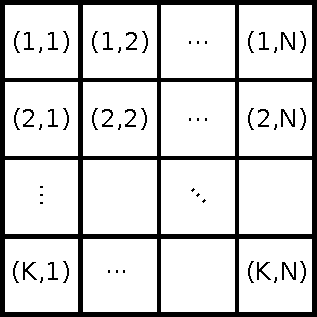
\includegraphics[width=\textwidth]{data_layouts.pdf}
      \caption{A simple 2-D data array with K rows and N columns.}
      \label{F:mem}
    \end{subfigure}
  \end{minipage}
  \hfil
  \begin{minipage}{0.45\linewidth}
    \begin{subfigure}[t]{\textwidth}
	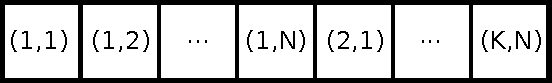
\includegraphics[width=\textwidth]{row_major.pdf}
	\caption{Row-major data ordering}
	\label{F:row_major}
    \end{subfigure}
    \\
    \begin{subfigure}[t]{\textwidth}
	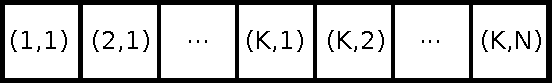
\includegraphics[width=\textwidth]{column_major.pdf}
	\caption{Column-major data ordering}
	\label{F:column_major}
    \end{subfigure}
  \end{minipage}
\end{figure}

When storing arrays for a chemical kinetic model, the data-storage layout and vectorization patterns are critical to achieving high-performance code.
\Cref{F:mem} depicts an example data array with K-rows and N-columns, with index ($i$, $j$) corresponding to the $i$th row and $j$th column.
For example the concentration of species $j$ for the $i$th thermo-chemical state would be stored in $[C]_{i, j}$ with $1 \le i \le N_{state}$, the number of thermo-chemical states considered for evaluation, and $1 \le j \le \ns/$, the number of species in the model.
The stored concentrations would then have $K = N_{\text{state}}$ rows, and $N = N_{\text{sp}}$ columns.

In the ``C'' (C row-major) format, the concentrations of all species for a single thermo-chemical condition $i$ would be stored sequentially in memory, i.e., with  $[C]_{1, 1}$ in index \num{1}, $[C]_{1, 2}$ in index \num{2} etc., as shown in \cref{F:row_major}.
Conversely in the ``F'' (Fortran column-major) format, the concentrations of a single species $j$ over all thermo-chemical states are adjacent in memory, corresponding to storing $[C]_{1, 1}$ in index \num{1}, $[C]_{2, 1}$ in index \num{2} and so on, as shown in \cref{F:column_major}.
This ordering---along with the device (CPU, GPU, etc.\@) and vectorization pattern in question---have a large effect on the performance of SIMD\slash SIMT-vectorized algorithms.

In a \textit{shallow}-SIMD\slash SIMT vectorization (also referred to as ``per-thread'' in previous works~\cite{Stone:2013aa} using GPUs), each SIMD-lane (or SIMT-thread) in a compute-unit evaluates the thermo-chemical source-terms\slash chemical kinetic Jacobian for a different thermo-chemical state.
If the data is stored in ``F''-order, the SIMD-lanes\slash SIMT-thread accessing $[C]_{1, j}\ldots[C]_{N_v, j}$---the concentration of species $j$ for states $1, 2,\ldots N_v$, where $N_v$ is the SIMD vector-width or the number of threads in a SIMT warp---will load sequential locations in memory.
The first $(j+1)$th species concentration, $[C]_{1, j+1}$, will be $N_{\text{state}}$ memory locations away; this increases the likelihood of cache-misses on the CPU~\cite{gray2000rules}, but conversely is well suited to coalesced memory accesses on the GPU~\cite{NVIDIA:2018}.

In a \textit{deep}-SIMD\slash SIMT vectorization (also referred to as ``per-block'' in previous GPU works), a compute-unit utilizes its SIMD-lanes\slash SIMT-threads cooperatively to evaluate the thermo-chemical source-terms for a single thermo-chemical state; thus SIMD-lanes loading $[C]_{1, j} \ldots [C]_{1, j + N_v}$---the species concentrations for state 1, species $j \ldots j + N_v$---will access sequential memory locations if the data is stored in ``C''-order.
Further, in the ``C''-ordering the furthest difference between any two species concentrations within the same thermo-chemical state is at most $N_{\text{sp}}$, with $N_{\text{sp}} \ll N_{\text{state}}$ in most cases; this greatly improved data-locality increases the chances of a cache-hit on the CPU, but may lead to uncoalesced memory-accesses on the GPU.
In addition, a deep vectorization requires both synchronization between SIMD-lanes\slash SIMT-threads via memory-fences\slash barriers (an expensive operation), and may result in SIMD-waste\slash SIMT thread-divergence, caused by different SIMD-lanes\slash SIMT-threads executing different instructions (e.g., resulting from different if\slash then branches)

\begin{figure}[htb]
  \centering
  \begin{minipage}{0.6\linewidth}
    \begin{subfigure}[t]{\textwidth}
	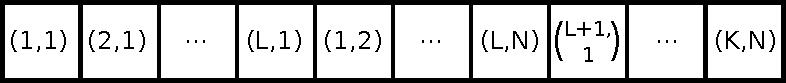
\includegraphics[width=\textwidth]{row_major_split.pdf}
	\caption{Row-major, shallow-vectorized data ordering}
	\label{F:row_major_split}
    \end{subfigure}
    \\
    \begin{subfigure}[t]{\textwidth}
	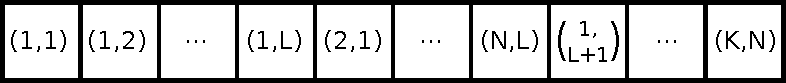
\includegraphics[width=\textwidth]{column_major_split.pdf}
	\caption{Column-major, deep-vectorized data ordering}
	\label{F:column_major_split}
    \end{subfigure}
  \end{minipage}
  \caption{Vectorized data ordering patterns}
  \label{F:vector_data}
\end{figure}

Finally,~\cref{F:vector_data} shows a vectorized data-ordering that improves the caching patterns of a shallow, ``C''-ordered SIMD vectorization on the CPU (\cref{F:row_major_split}) and a deep, ``F''-ordered SIMT vectorization on the GPU (\cref{F:column_major_split}).
This is accomplished by splitting the slower-varying axis of the data array---columns for ``C''-ordering, and rows for ``F''-ordering---into chunks of size $N_v$ (the SIMD vector-width, or SIMT warp-size) and laying these data out contiguously in memory.
For example, using the shallow-vectorized ``C''-ordering pictured in~\cref{F:row_major_split}, the concentration of species $j$ for states $i\ldots i+N_v$, $[C]_{i, j} \ldots [C]_{i + N_v, j}$, are contiguous in memory and are followed by the concentration of species $j + 1$ for the same states, $[C]_{i, j + 1} \ldots [C]_{i + N_v, j + 1}$.
This pattern, similar to OpenCL's native vector data-types---e.g., \texttt{double\num{8}} which treats \num{8} contiguous double precision floating point numbers as a single vector datum---ensures that any SIMD operation occurs on data that is contiguous in memory, greatly improving caching and SIMD-throughput.
Conversely, the data-ordering in~\cref{F:column_major_split} is designed to enable coalesced memory accesses for ``F''-ordered, deep-SIMT vectorization on the GPU.
The effects of these various data-ordering and vectorization patterns on performance will be studied in~\cref{S:results}.

\subsection{Thermo-chemical Source-Terms and Jacobian}
This new version of \texttt{pyJac} is capable of evaluating the thermo-chemical source-terms for using both the constant-pressure (\conp/) or constant-volume (\conv/) assumption\footnote{Note: in this context, the ``constant-pressure'' and ``constant-volume'' assumptions refer to evaluation within a reaction sub-step in the operator splitting scheme, rather than a general constant-pressure or constant-volume reactive-flow simulation.}
In this section, we will only outline a brief summary of the system evaluated by \texttt{pyJac}; the interested reader is referred to the complete derivations, attached as supplemental material to this document.


The thermo-chemical state vector derivation consists of the temperature, a non-constant thermodynamic state parameter (volume or pressure for \conp/ and \conv/ respectively), and the number of moles of all species except the last species in the chemical model which is typically taken to be the bath-gas (e.g., \ce{N2}):
\loadeq{state}
where $T$ is the temperature, $V$ and $P$ the volume and pressure respectively, and $n_j$ the number of moles of the $j$th species in the model (containing $\ns/$ total species).

This state vector---inspired by~\cite{SCHWER2002270}---has a number of features that recommend its use.
First, the state vector results in highly sparse chemical kinetic Jacobians as will be detailed in~\cref{S:sparsity}.
Second, mass is explicitly conserved in this formulation owing to the fact that the moles of the final species is calculated from the ideal gas law, and the rate of change of the final species from conservation of mass (see \cref{deriv-s:state,deriv-s:source} of the supplemental material respectively); additionally, system is not over-constrained and does not require use of a more complicated DAE solver (as compared to an ODE integrator) for integration\todo{hansen citation here}.
Finally, the chemical kinetic Jacobian changes relatively little between the \conp/ and \conv/ forms, making maintaining the code-base much simpler.
Although most current combustion codes do not use species moles as a state variable, conversion to\slash from more common mass\slash mole-fractions and moles is straightforward, and once inside integration of an chemical kinetic initial value problem (IVP), the choice of variables no longer matter.

The evolution of the thermo-chemical state vector is described by a set of chemical kinetic ordinary differential equations:
\loadeq{dstate}

For both \conp/ and \conv/, the molar source-terms are~\cite{TurnsStephenR2012Aitc}:
\loadeq{dmolar}
where $\dot{\omega}_k$ is the $kth$ species' overall production rate:
\begin{equation}
 \dot{\omega}_{k} = \sum_{i=1}^{\nr/} \nu_{k, i} R_{i} c_{i}
\end{equation}
with $\nu_{k, i}$ the net stoichiometic coefficient of species $k$ in reaction $i$, $R_{i}$ the net rate of progress of reaction $i$ (described in~\cref{deriv-s:rop_net} of the supplemental), and $c_{i}$ the pressure modification term i.e., for third-body (see~\cref{deriv-s:thdbody} of the supplemental), or fall-off\slash chemically-activated reactions (\cref{deriv-s:falloff} of the same).

The temperature source-term~\cite{TurnsStephenR2012Aitc} is:
\loadeq{dtemp}
where $H_k$, $U_k$, $C_{p,k}$ and $C_{v, k}$ are the enthalpy, internal energy, constant-pressure and constant-volume specific heat of species $k$ in molar units respectively, while $[C]_{k}$ is the concentration, given by:
\begin{equation}
 [C]_{k} = \frac{n_{k}}{V}
\end{equation}
By differentiating the ideal gas law:
\begin{equation}
 PV = n\mathcal{R}T \;,
\end{equation}
where $\mathcal{R}$ is the ideal gas-constant in molar units, the volume and pressure source-terms can be found:
\loadeq{dparam}

The Jacobian entries computed by \texttt{pyJac} are arranged such that entry ($i$, $j$) corresponds to the partial derivative of the $i$th source-term in~\cref{e:source_terms} by the $j$th state variable in~\cref{e:state}:
\loadeq{jacgeneral}

The derivative of the temperature source-term with respect to itself is:
\loadeq{dTdotdT}
and with respect to the thermodynamic state parameter (the volume \slash pressure for \conp/\slash\conv/ respectively):
\loadeq{dTdotdE}
and the moles of species $j$:
\loadeq{dTdotdnj}

The derivative of the thermodynamic state parameter with respect to the temperature is:
\loadeq{dEdotdT}
and with respect to itself:
\loadeq{dEdotdE}
and finally, by the moles of species $j$:
\loadeq{dEdotdnj}

The molar source-terms are more complicated due to the derivatives of the net rate of progress---see~\cref{deriv-s:dropi}---and pressure modification terms---\cref{deriv-s:dci}---of the reactions.
The reader is again encouraged to read the supplemental material covering the exact derivations and equations solved by \texttt{pyJac}.
The derivative of the molar source-term with respect to temperature is:
\loadeq{dnkdotdT}
while, similarly the derivative with respect to the state parameter is:
\loadeq{dnkdotdE}
and the moles of species $j$:
\loadeq{dnkdotdnj}

\subsection{Code Generation and Testing Infrastructure}
\label{s:unittest}
Code generation is enabled by the python package \texttt{loo.py}~\cite{kloeckner_loopy_2014}, which translates user specified pseudo-code and data to OpenCL\slash C-code.
As the name implies, \texttt{loo.py} generates code based on for-loops, this differs from the previous version of \texttt{pyJac}~\cite{pyjac16} which generates static code (i.e., fully unrolled loops, with thermodynamic\slash reaction parameters written directly in code rather than stored in arrays).
In our previous work,~\cite{Niemeyer:2016aa} this static code generation caused some issues with large file sizes, long compilation times and even occasionally breaking the \texttt{gcc} and \texttt{nvcc} compilers (the latter issue necessitated breaking the Jacobian\slash source-term evaluations into separate files).
The implications of this change will be studied in~\cref{S:jacobian_results}, where the performance of the new version of~\texttt{pyJac} will be compared to the previous versions.

In addition, \texttt{loo.py} allows the user to more easily make changes the structure of the generated program, e.g., data ordering, vectorization, and threading patterns, as well as switching the target-language for code-generation (and simpler extension to additional languages, e.g., CUDA).
Further, \texttt{loo.py} can execute developed subroutines from python (natively for C-code, or via \texttt{PyOpenCL}~\cite{kloeckner_pycuda_2012} for OpenCL-code), enabling unit-testing\slash validation for each component of the Jacobian or source-terms.
The source-terms and sub-components thereof (e.g., rates of progress, pressure-modification terms, etc.) are directly compared to Cantera~\cite{Cantera}, while the automatic differentiation code Adept~\cite{hogan2014fast,adept-v11} is used to obtain reference answers for Jacobian sub-components.
The Portable OpenCL (POCL) implementation~\cite{poclIJPP} and OpenMP~\cite{dagum1998openmp} are used to run OpenCL and C unit-testing, respectively, on the continuous integration framework Travis CI~\cite{travis:2018}.
Validation of the complete (as opposed to the sub-component testing discussed here) generated source-terms and Jacobian codes will be discussed in detail in~\cref{s:validation}.


\section{Results and Discussion}
\subsection{Testing platforms}

\begin{table}[htb]
\centering
\begin{tabular}{@{}l l l@{}}
\toprule
CPU Model        & Xeon X5650      & E5-2690 V3     \\
\midrule
Instruction Set  & SSE4.2 	   & AVX2 	    \\
Vector Width     & \SI{2}{\doubles}&\SI{4}{\doubles}\\
Cores            & $2 \times 6$    & $2 \times 12$  \\
Identifier       & \sse/ 	   & \avx/  	    \\
OpenCL Version   & \num{1.2}       & \num{1.2}      \\
\bottomrule
\end{tabular}
\caption{The Intel CPU configurations used in this study.
	 The vector-width reported in this table is reported in (ideal) number of double operations per SIMD instruction, as this will be used in measuring SIMD efficiency; for reference, the vector-width in bits of the \sse/ and \avx/ machines are \SI{128}{\bit} and \SI{256}{\bit} respectively.
	 The identifier field will be used as a shorthand descriptor in the performance plots to quickly identify the CPU type.}
\label{t:cpus}
\end{table}

The performance and validation studies for this work were run on a variety of CPU and GPU platforms.
\Cref{t:cpus} shows the number of cores, vector instruction set and model of the CPUs used in this work; each CPU had both \texttt{v16.1.1} of the Intel OpenCL runtime~\cite{intelopencl:2018} and \texttt{v1.0} of the POCL~\cite{poclIJPP} runtime installed, each enabling OpenCL \texttt{v1.2} execution.
Additionally, \texttt{v5.0} of the LLVM\slash\texttt{clang}~\cite{Lattner:2004:LCF:977395.977673} compiler chain was installed on all machines to enable use of POCL.
\Cref{t:gpus} lists the model, number of CUDA cores and NVIDIA driver of each of the GPUs used in this work.
NVIDIA's OpenCL runtime is bundled with the NVIDIA driver~\cite{NVIDIA:2018}, hence we the driver version is used to specify the OpenCL runtime version.

\begin{table}[htb]
\centering
\begin{tabular}{@{}l l l l l@{}}
\toprule
NVIDIA Model   & Tesla C2075    & Tesla K40m    \\
\midrule
Driver Version & \num{384.81}   & \num{387.26}  \\
CUDA Cores     & \num{448}      & \num{2880}    \\
Identifier     & \gpuold/ 	& \gpunew/	\\
OpenCL Version & \num{1.1}	& \num{1.2}	\\
\addtocounter{footnote}{1}
Memory\footnotemark[\thefootnote] & \SI{6}{\giga\byte} & \SI{12}{\giga\byte} \\
\bottomrule
\end{tabular}
\caption{The NVIDIA GPU configurations used in this study.  NVIDIA's OpenCL runtime is provided with the graphic driver, rather than any specific version of CUDA.
Again, the identifier field will be used as a shorthand descriptor during analysis of the performance results.
}
\label{t:gpus}
\end{table}
\footnotetext{Due to an driver implementation issue~\cite{nvidia_memory}, the total memory used on the \gpuold/ and \gpunew/ GPUs were to limited to \SI{4}{\giga\byte} and \SI{10}{\giga\byte} respectively.\addtocounter{footnote}{1}}


\Cref{t:platforms} lists the platforms and vectorization\slash execution patterns they are capable of running.
The Intel and NVIDIA OpenCL runtimes lack implementations of atomic operations on double precision variables; these are currently necessary for \texttt{pyJac} to run deep-vectorized code.
On the other hand, POCL is an open source OpenCL runtime that works on all CPU types tested in this work, and does implement these atomic operations.
However, POCL's implicit vectorization module---which utilizes the LLVM compiler~\cite{Lattner:2004:LCF:977395.977673} to translate OpenCL code to vectorized machine code---typically fails to achieve much speedup, if any.
Thus POCL is a particularly useful tool for validation, but not necessarily for performance studies.
This discussion will be expanded upon in~\cref{s:future} to highlight the most promising future directions.

\begin{table}[htb]
\centering
\begin{tabular}{@{}l c c c@{}}
\toprule
Platform & Parallel & Shallow Vectorization & Deep Vectorization \\
\midrule
OpenMP & X & -- & -- \\
POCL OpenCL & X & X & X \\
Intel OpenCL & X & X & -- \\
NVIDIA OpenCL & -- & X & -- \\
\bottomrule
\end{tabular}
\caption{The various platforms used in this study and the execution \slash vectorization patterns they are capable of running}
\label{t:platforms}
\end{table}

Finally, \cref{t:models} displays the chemical kinetic models used in this work, as well as number of partially stirred reaction conditions (PaSR) in the condition database for each.
Creation of the PaSR databases are described in detail our previous works~\cite{CurtisGPU:2017,Niemeyer:2016aa}.

\begin{table}[htb]
\centering
\begin{tabular}{@{}l c c @{}}
\toprule
Model &  Number of Conditions & Reference \\
\midrule
\ce{H2}\slash\ce{CO} & \num{900900} & \cite{Burke:2011fh} \\
GRI-Mech.~3.0         & \num{450900} & \cite{smith_gri-mech_30} \\
USC-Mech II           & \num{91800}  & \cite{Wang:2007} \\
\ce{iC5H11OH}         & \num{450900} & \cite{Sarathy:2013jr} \\
\bottomrule
\end{tabular}
\caption{The chemical kinetic models used in this study and number of conditions in the partially stirred reactor database for each.}
\label{t:models}
\end{table}


\subsection{Source-term validation}
\label{s:validation}
The reaction rates of progress (ROP), species and temperature rates in this study are validated by comparison with Cantera~\cite{Cantera}, however special care must be taken due floating point arithmetic issues.

For a direct comparison, a relative error norm of a quantity $X_{ij}$ over all states $j$, and reactions (or species) $i$ was computed using the $L^{\infty}$ norm:
\begin{equation}
E_{X} = \left\lVert \frac{\left\lvert X_{ij,\text{CT}} - X_{ij}\right\rvert}{\num{e-10} + \num{e-6} * \left\lvert X_{ij,\text{CT}} \right\rvert} \right\rVert_{i,j,\infty}
\label{e:rel_err}
\end{equation}
where the \text{CT} subscript indicates values from Cantera~\cite{Cantera}

However, in computing the net ROP of reaction $i$ for state $j$ from the forward and reverse ROP: $R_{ij} = R_{ij}^{\prime} - R_{ij}^{\prime\prime}$, accuracy can easily be lost as the net ROP may be---particularly near chemical equilibrium---many orders of magnitude smaller than the forward or reverse rates.
To quantify this phenomena, the error in forward ROP is first defined as:
\begin{equation}
\varepsilon^{\prime}_{ij} = \left\lvert R_{ij}^{\prime} - R_{ij,\text{CT}}^{\prime} \right\rvert
\end{equation}
while the error in reverse ROP, $\varepsilon^{\prime\prime}_{ij}$, can be defined analogously.
Finally, for the reaction $i^{*}$ and state $j^{*}$ that result in the largest error in net ROP, i.e. $E_{R}$, an estimate of the error attributable to floating point error accumulation from the forward and reverse ROPs can be obtained as:
\begin{equation}
E_{\varepsilon} = \frac{\max(\varepsilon^{\prime}_{i^{*}j^{*}}\text{, }\varepsilon^{\prime\prime}_{i^{*}j^{*}})}{\num{e-10} + \num{e-6} * \left\lvert R_{i^{*}j^{*},\text{CT}} \right\rvert}
\end{equation}
This estimate allows for direct comparison of the error in forward or reverse ROPs to the value of the net ROP itself, if they are of similar magnitude the error in net ROP will be large.

\begin{table}[htbp]
\sisetup{retain-zero-exponent=true}
\centering
\begin{tabular}{@{}l S[table-format=1.2e1] S[table-format=1.2e1] S[table-format=1.2e1] S[table-format=1.2e1]@{}}
\toprule
\multicolumn{1}{l}{Model} & \multicolumn{1}{l}{\ce{H2}\slash\ce{CO}} & \multicolumn{1}{l}{GRI-Mech.~3.0} & \multicolumn{1}{l}{USC-Mech II} & \multicolumn{1}{l}{\ce{iC5H11OH}} \\
\midrule
\multicolumn{1}{c}{$E_{R^{\prime}}$}                    & 1.56e-8 & 2.95e-8 & 9.42e-8 & 4.86e-4 \\
\multicolumn{1}{c}{$E_{R^{\prime\prime}}$}              & 6.92e-8 & 6.53e-8 & 1.20e-7 & 5.07e-4 \\
\multicolumn{1}{c}{$E_{R}$}                             & 1.49e1  & 1.11e0  & 2.80e0  & 4.82e-1 \\
\multicolumn{1}{c}{$E_{\varepsilon}$}                   & 1.48e1  & 1.13e0  & 2.93e0  & 5.03e-1 \\
\multicolumn{1}{c}{$E_{\frac{\text{d} n}{\text{d} t}}$} & 2.53e1  & 2.60e0  & 7.62e0  & 1.58e1 \\
\multicolumn{1}{c}{$E_{\frac{\text{d} T}{\text{d} t}}$} & 3.94e5  & 3.35e8  & 3.95e6  & 7.11e7 \\
\multicolumn{1}{c}{$E_{\frac{\text{d} S}{\text{d} t}}$} & 3.52e12 & 3.46e12 & 3.44e12 & 3.38e12 \\
\bottomrule
\end{tabular}
\caption{Summary of rate of progress, species, temperature and thermodynamic state parameter rate correctness.
Error statistics are based on the infinity-norm of the relative error detailed in~\cref{e:rel_err} for each quantity.
The ``S'' in $E_{\frac{\text{d} S}{\text{d} t}}$ refers to the thermodynamic state parameter, either $V$ or $P$ for \conp/ and \conv/ respectively.
}
\label{T:source_error}
\end{table}

In Table~\ref{T:source_error}, the results of this code's source-term evaluations are compared to Cantera~\cite{Cantera} on the library of PaSR conditions (\cref{t:models}).
Very close agreement is observed for the forward and reverse ROP for all models, however the error norm is \textasciitilde\numrange{3}{4} orders of magnitude larger for the isopentanol model.
This results from differences in evaluation of P-Log reactions between \texttt{pyJac} and Cantera; namely \texttt{pyJac} computes the logarithm of the upper and lower reaction Arrhenius rates (see supplemental~\cref{deriv-s:pdep}) analytically while Cantera evaluates this term numerically.
If the error from P-Log reactions are not considered in~\cref{e:rel_err}, the forward and reverse ROP falls to \num{5.44e-08} and \num{1.59e-07} respectively.
We note that this discrepancy does not imply any incorrectness in either \texttt{pyJac} or Cantera---in fact, the error is still well within the proscribed tolerances in~\cref{e:rel_err}---but merely emphasizes the effect small code-changes can have on the accumulation of floating point errors.

This point is further underscored by the error in the net ROP, which is \textasciitilde\numrange{3}{9} orders of magnitude (or \numrange{7}{9} orders of magnitude for the P-Log excluded error) larger than the error in either the forward or reverse ROP.
In~\cref{T:source_error}, it is seen that $E_{\varepsilon}$ is very similar in magnitude to $E_R$ in all cases, indicating that this large increase in error is caused by the accumulation of floating point error from the forward and reverse ROPs, as previously discussed.
The molar species production rate error norm is similar in magnitude to that of the net ROP, however the temperature and state parameter rate errors again increase as the error in net species production rates is amplified by multiplication with thermodynamic properties.
Again, we note that the above discussion does not imply that discrepancies in computation of the net ROP will cause large error in chemical kinetic integration---either in this code or Cantera~\cite{Cantera}---as this loss of accuracy only occurs when the forward and reverse ROP are nearly equal, implying the reaction is in near-equilibrium.

\subsection{Jacobian validation}

As in our previous work~\cite{Niemeyer:2016aa}, the correctness of the Jacobian was determined by comparison to the Jacobian obtained by automatic differentiation of the source-term subroutines generated by \texttt{pyJac} via the \texttt{Adept} software library~\cite{adept-v11,hogan2014fast}.
The reasons for this choice are explained fully in~\cite{Niemeyer:2016aa}, but broadly speaking automatic differentiation provides relatively fast, highly accurate Jacobian matrix evaluation with minimal additional programming effort.
The discrepancy between the analytical and automatic differentiated Jacobians for thermo-chemical state $k$, denoted by $\mathcal{J}_k$ and $\hat{\mathcal{J}}_k$ respectively, is determined by the relative error Frobenius norm over all Jacobian indices $i, j$:
\begin{equation}
 \label{e:jac_error_base}
 E_{\text{rel}, k} = \left\lVert \frac{\hat{\mathcal{J}}_{ijk} - \mathcal{J}_{ijk}}{\hat{\mathcal{J}}_{ijk}} \right\rVert_{i,j,F}
\end{equation}

To avoid large relative errors of very small nonzero Jacobian elements due to accumulation of floating point error, the Frobenius norm of the automatically differentiated Jacobian is calculated over all thermo-chemical states $k$:
\begin{equation}
 \label{e:thresh}
 \mathcal{T} = \left\lVert \mathcal{\hat{J}} \right\rVert_{k, F}
\end{equation}
The error statistics reported in this section are then based only on matrix elements where $\mathcal{J}_{ijk} \ge \frac{\mathcal{T}}{\mathcal{C}}$; this filtered form of~\cref{e:jac_error_base} is denoted $E_{\mathcal{C},k}$.
Finally, the Frobenius norm is calculated over all the states in the PaSR thermo-chemical condition database:
\begin{equation}
 \label{e:thresholded_error}
 E_{\mathcal{C}} = \left\lVert E_{\mathcal{C},k} \right\rVert_{k, F}
\end{equation}

It is noted that this error norm is quite different from the relative error Frobenius norm suggested by Anderson et al.~\cite{Anderson:1999aa} for quantifying the error of matrices in LAPACK:
\begin{align}
 \label{e:error_lapack}
 \lhs{lapack}{E_{\mathcal{L}, k}} &=  \rhs{lapack}{\frac{\left\lVert \hat{\mathcal{J}}_{ijk} - \mathcal{J}_{ijk} \right\rVert_{i,j,F}}{\left\lVert \hat{\mathcal{J}}_{ijk} \right\rVert_{i,j,F}}} \nonumber \\
 \lhs{lapack}{E_{\mathcal{L}}} &= \rhs{lapack}{\left\lVert  E_{\mathcal{L}, k} \right\rVert_{k, F}}[c]
\end{align}
In our experience, the LAPACK error norm is often dominated by the accuracy of the larger elements in the Jacobian, while the filtered error norm is useful for identifying errors in both large and small Jacobian entries.
Further, with a tunable threshold parameter, $\mathcal{C}$, the error of different ranges of of element sizes can be assessed, and the effects of floating point error can be isolated.
For reference, both our own error norm and the LAPACK error norm will be reported.

\begin{table}[htbp]
\sisetup{retain-zero-exponent=true}
\centering
\begin{tabular}{@{}l S[table-format=.0] S[table-format=1.3e1] S[table-format=1.3e1] S[table-format=1.3e1] S[table-format=1.3e1] @{}}
\toprule
Model                 & \multicolumn{1}{c}{$E_{\mathcal{L}}$} & \multicolumn{1}{c}{$\bar{\mathcal{T}}$} & \multicolumn{1}{c}{$E_{\mathcal{C} = 10^{20}}$}   & \multicolumn{1}{c}{$E_{\mathcal{C} = 10^{15}}$} \\
\midrule
\ce{H2}\slash \ce{CO} & \num{1.048e-11}      & \num{6.431e+18}      & \num{1.741e+0}  & \num{4.508e-5} \\
GRI-Mech 3.0          & \num{1.124e-14}      & \num{7.783e+19}      & \num{3.842e-7}  & \num{3.687e-7} \\
USC-Mech II           & \num{9.632e-15}      & \num{2.830e+21}      & \num{1.119e-2}  & \num{1.983e-7} \\
\ce{iC5H11OH}         & \num{1.227e-10}      & \num{2.733e+26}      & \num{1.363e-3}  & \num{2.764e-5} \\
\bottomrule
\end{tabular}
\caption{Summary of Jacobian matrix validation results.
Error statistics are the largest filtered relative error $E_\mathcal{C}$ for over all test platforms, vectorization patterns (\cref{t:platforms}),  \conp/\slash \conv/ and sparse\slash dense Jacobians.
It is noted that the threshold described in~\cref{e:thresh} varies slightly between the \conp/ and \conv/ cases; the reported $\bar{\mathcal{T}}$ is the average of the two, however the appropriate value was used during calculations of the error statistics.
}
\label{T:error}
\end{table}

\Cref{T:error} reports the maximum $E_{\mathcal{C}}$ and $E_{\mathcal{L}}$ values over all test platforms\slash vectorization patterns (see~\cref{t:platforms}), sparse\slash dense (see~\cref{S:sparsity}) and \conp/\slash\conv/ Jacobians.
The most stringent filtered error norm ($\mathcal{C} = 10^{20}$) ranges from \numrange[retain-zero-exponent=true]{e-7}{e0}; the largest error is for the \ce{H2}\slash\ce{CO} model.
For this model, $\mathcal{T}$  is smaller than the tolerance of \num{e20}, and hence the error norm considers Jacobian entries smaller than $\mathcal{O}(1)$.
It is noted that for GRI-Mech 3.0, which has a $\mathcal{T}$ roughly an order of magnitude larger, the stringent error norm is significantly smaller: $\mathcal{O}(\num{e-7})$.
Given the intricacy of floating point error evaluation, the use of different languages and OpenCL platforms (the effect of these differences will be explored in Appendix \textbf{???}\todo{this}), and the general complexity of \texttt{pyJac} it would be exceedingly difficult to pinpoint an exact cause for this phenomena, as was done in~\cref{s:validation}.
To ensure there is no bug or error present in the Jacobians generated by \texttt{pyJac}, a relaxed filtered error norm ($\mathcal{C} = 10^{15}$) is also presented for each model in~\cref{T:error}.
This relaxed norm is smaller by \numrange{2}{5} orders of magnitude for all models---except GRI-Mech 3.0, where the stringent case has very small error as previously discussed---indicating that accuracy is higher when the smaller Jacobian entries are excluded; this suggests floating point error accumulation is the primary driver of the stringent filtered error norm.

The relative LAPACK error norm---ranging from \textasciitilde\numrange{e-10}{e-14}---re-enforces this finding, as it indicates roughly \numrange{10}{14} digits of accuracy~\cite{Anderson:1999aa}.
Further, the LAPACK error norm does not correlate well with the stringent filtered error norm, e.g., USC-Mech II has the lowest LAPACK error norm (\num{9.632e-15}), but the second largest stringent filtered error norm (\num{1.119e-2}).
Conversely, the LAPACK error norm does seem to correlate with the relaxed filtered error norm; the two models with the largest LAPACK error, \ce{H2}\slash\ce{CO} and \ce{iC5H11OH}, have the largest relaxed filtered error norms, $\mathcal{O}(\num{e-5})$, again suggesting that the stringent error norm is influenced by floating point error accumulation.
These findings, along with the individual unit-testing of all chemical source-terms and Jacobian sub-components described in~\cref{s:unittest}, gives high confidence in the correctness of this new version of \texttt{pyJac}.


\subsection{Sparsity patterns}
\label{S:sparsity}

In general, the Jacobian matrices generated by \texttt{pyJac} are largely sparse with non-zero entries corresponding mainly to species that participate in the same reaction (or non-default efficiency third-body species in a reaction), and mostly dense rows\slash columns corresponding to the temperature and thermodynamic state parameter.
However, the explicit-mass conservation formulation of \texttt{pyJac} can introduce additional non-zero entries in two ways.
First, if the last-species in the model (i.e., the bath-gas) participates directly in a reaction, the derivative of the forward or reverse rate of progress with respect to any other species is non-zero (see~\cref{deriv-s:dri_dnj} of the supplemental).
Similarly, if the last-species has a third-body efficiency not equal to the default (unity), this will again force all the derivative of the pressure-modification term with respect to other species to be non-zero (see~\cref{deriv-s:dci_thd} of the same).
Either case will result in an undesirable fully dense Jacobian row for all species that have a non-zero net stoichiometic coefficient in such a reaction.

However, \texttt{pyJac} allows the user to simply ignore these derivatives (via a command-line switch) and avoid any negative adverse affects on the Jacobian sparsity.
The rational behind this choice is that many common implicit integration techniques (e.g., CVODE~\cite{Hindmarsh:2005}) used in solution of chemical kinetic initial value problems are formulated around the assumption that the supplied Jacobian is approximate; this allows the Jacobian and its LU factorization to be reused for multiple internal integration time-steps, accelerating the solution process.
For such solvers, there is no need for the exact form of the Jacobian and the so-called ``approximate'' form is preferable.
Hence, in this section we will detail the sparsity of both forms of the Jacobian for the chemical models tested.

In~\cref{F:jac_sparsity}, a graphical representation of the sparsity pattern for GRI-Mech 3.0 is displayed.
In particular we note that~\cref{F:jac_sparse_approx} is has several rows that are no longer fully-dense, as result of its approximate form; these rows correspond to species directly interacting with \ce{N2}, largely in GRI-Mech 3.0's \ce{NOx} chemistry reactions.
\cref{T:jac_sparsity} shows the density of the exact and approximate Jacobians for all mechanisms tested in this work.
The smallest model, \ce{H2}\slash\ce{CO} is very dense with \textasciitilde\SI{70}{\percent} of the Jacobian entries non-zero, however this drops to \textasciitilde\SI{50}{\percent} for GRI-Mech 3.0, and continues to decrease to \textasciitilde\SI{27}{\percent} for USC-Mech II and just \textasciitilde\SI{10}{\percent} for the isopentanol model.
The approximate Jacobian assumption drops the density of Jacobian by \textasciitilde\SIrange{3}{7}{\percent} for all models.

\begin{figure}[htb]
  \centering
  \begin{subfigure}[t]{0.48\linewidth}
      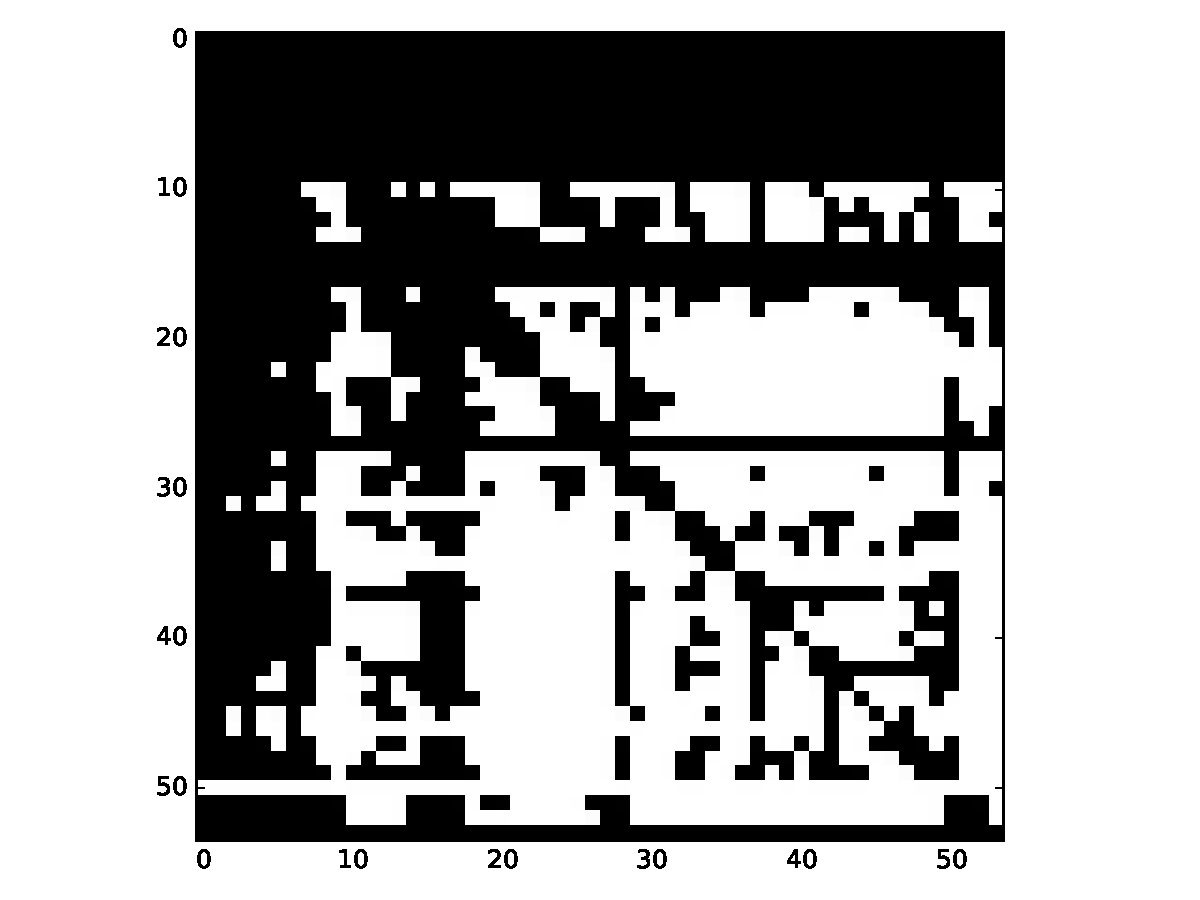
\includegraphics[width=\textwidth]{ch4_sparsity_exact.pdf}
      \caption{The ``exact'' Jacobian.}
      \label{F:jac_sparse_exact}
  \end{subfigure}
  \hfill
  \begin{subfigure}[t]{0.48\linewidth}
      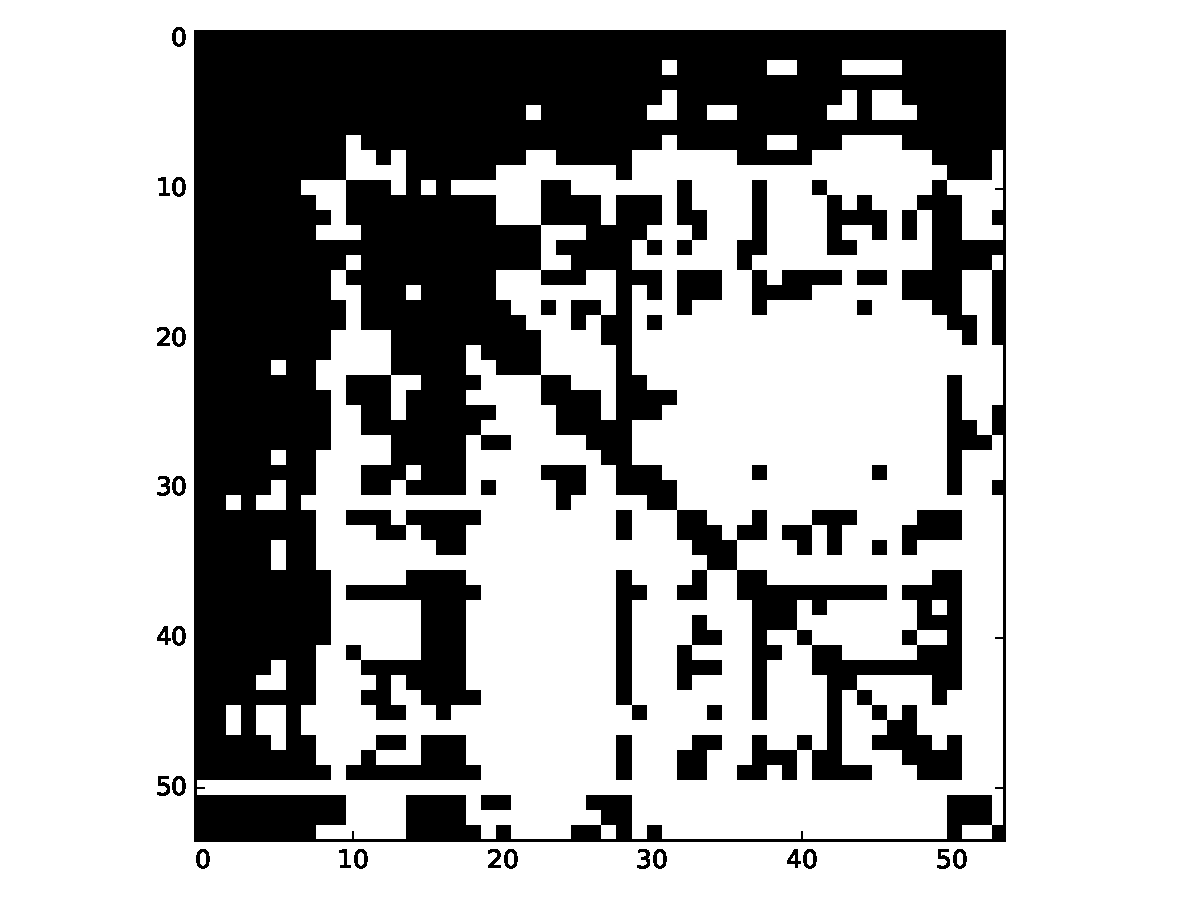
\includegraphics[width=\textwidth]{ch4_sparsity_approximate.pdf}
      \caption{The ``approximate'' Jacobian.}
      \label{F:jac_sparse_approx}
  \end{subfigure}
  \caption{A graphical representation of the sparsity pattern of the chemical kinetic Jacobian generated by \texttt{pyJac} for GRI-Mech 3.0.
	   Black squares indicate a non-zero Jacobian entry, while white square correspond to an empty entry.
	   The numbers indicate the index of the entry in the state vector.}
  \label{F:jac_sparsity}
\end{figure}

Currently, \texttt{pyJac} can utilize two common sparse matrix storage formats~\cite{netlib_templates}, compressed row\slash column storage (CSR\slash CSC), used for ``C'' and ``F''-ordered data respectively.
For convenience we will outline only the CSR format but the CSC format is very similar~\cite{netlib_templates}.
An $N\times N$ CSR matrix is composed of three vectors, a value vector of length $NNZ$---the number of non-zero elements in the Jacobian---which stores the elements of the Jacobian, a row pointer vector---of length $N$---which stores the locations in the value vector that begin a row, and a column index vector---of length $NNZ$---which stores the column indices of the elements in the value vector.

\begin{table}[tbp]
\centering
\begin{tabular}{@{}l S[table-format=2.1] S[table-format=2.1]@{}}
\toprule
Model                 & \multicolumn{1}{c}{Exact Jacobian Density} & \multicolumn{1}{c}{Approximate Jacobian Density} \\
\midrule
\ce{H2}\slash \ce{CO} & \SI{71.4}{\percent} & \SI{68.4}{\percent} \\
GRI-Mech 3.0          & \SI{56.7}{\percent} & \SI{49.8}{\percent} \\
USC-Mech II           & \SI{28.2}{\percent} & \SI{26.4}{\percent} \\
\ce{iC5H11OH}         & \SI{11.5}{\percent} & \SI{7.98}{\percent} \\
\bottomrule
\end{tabular}
\caption{The density of the exact and approximate Jacobians generated by \texttt{pyJac} for the various models studied.}
\label{T:jac_sparsity}
\end{table}

The Jacobian access pattern used by \texttt{pyJac} is fairly irregular; for simplicity we will only discuss looping-structure of species derivatives calculations as these form the bulk of the computation, and have the most challenging Jacobian access patterns.
In general, an outer loop iterates over all reactions of a certain type (e.g., falloff reactions) and calculates the relevant Jacobian subproducts---independent of any particular species---for the reaction (e.g., the the derivative of the falloff pressure modification term).
Two inner loops then iterate over the species in a reaction, updating the Jacobian entries for these species as appropriate.
This pattern leads to fairly easily vectorizable code, and efficient Jacobian evaluation as the bulk of the computation is dependent only on the reaction in question, as discussed in our previous work~\cite{Niemeyer:2016aa}.
Generally, this means that a lookup operation is required to find the sparse Jacobian index for any pair of state variables; in some cases this can be avoided, e.g., the rows corresponding to derivatives of the temperature and thermodynamic state parameter source-terms are fully dense in \texttt{pyJac}, and hence no lookup is necessary.
This lookup operation is currently implemented as a simple for-loop, e.g., for a sparse lookup of a pair of indices $(i, j)$ in a compressed row storage matrix, the lookup function searches the column index vector between the values $\texttt{row\_pointer}[i] \ldots \texttt{row\_pointer}[i + 1]$ for $j$, and returns the offset from $\texttt{row\_pointer}[i]$ (or $\num{-1}$ if not found).
As will be explored in~\cref{S:jacobian_results}, this slows down sparse Jacobian evaluation, and might be improved---at the cost of increased constant data usage, a limitation for OpenCL---by a static mapping of the full Jacobian indices to the sparse index (or some null value if the entry is empty).
Additionally, this might be an excellent usage of OpenCL's Image memory type (similar to texture memory in CUDA terminology) and both of these sparse indexing techniques merit future investigation.


\subsection{Performance}
\label{S:results}
The performance studies in this work were run on the platforms listed in~\cref{t:cpus,t:gpus}.
Run times in each case were averaged over ten runs, each using the same set of PaSR conditions utilized in validation.
The OpenMP Jacobian\slash source-term kernels, as well as the OpenMP\slash OpenCL wrapping code---responsible for initializing\slash transferring memory, reading input, etc.---was compiled with \texttt{gcc v5.4.0} on the \avx/\slash\gpunew/ platforms, and \texttt{gcc v4.8.5} on the \sse/\slash\gpuold/ machines.
The optimization level ``\texttt{-O3 -mtune=native}'' was used, and no ``fast-math'' OpenCL optimizations were enabled.
Additionally, the exact form of the Jacobian (as opposed the the ``approximate'' form discussed in~\cref{S:sparsity}) was used in all cases.
Finally, unless stated otherwise: the performance results utilized the \conp/ assumption, a vector-width of \num{8}\slash\num{128} and ``C''\slash ``F''-ordered data for the CPU\slash GPU cases respectively; the run times reported are for the number of conditions specified in~\cref{T:error} and include data transfer overhead to\slash from internal buffers used in \texttt{pyJac}.
The effects of choice of vector-width, data-ordering and differences between \conp/ and \conv/ evaluations on the CPU\slash GPU will be explored in~\cref{S:source_results}.

\subsubsection{Source-term evaluation}
\label{S:source_results}

\Cref{F:cpu_source} explores the performance of the source-term evaluations generated by \texttt{pyJac} on the CPU test platforms listed in~\cref{t:cpus}.
Source-term evaluations---critical in their own right for direct numerical simulations of reacting flow~\cite{Spafford:2010aa}, among other applications---also give a convenient platform to detail the effects of various code configuration options before investigating the more involved Jacobian evaluation performance.

In~\cref{F:intel_source_nonorm}, the mean run time per initial condition is shown for both the~\avx/ and~\sse/ CPUs, using both Intel OpenCL and OpenMP.
This normalization of the run time by the number of initial conditions tested is chosen to account for the varying numbers of conditions in the PaSR databases for each model (\cref{t:models}).
For both CPUs, the OpenMP implementation is the slowest over all models; interestingly the unvectorized (strictly parallel) Intel OpenCL code is slightly faster than OpenMP in all cases.
As expected, the \avx/ machine is faster than the \sse/ CPU for the strictly parallel cases, \SIrange{1.82}{2.13}{$\times$} for the unvectorized OpenCL case, and \SIrange{1.72}{1.85}{$\times$} for OpenMP.
Additionally, the shallow-vectorized OpenCL code is significantly faster than either the OpenMP or unvectorized OpenCL codes on both processors.

\begin{figure}[htbp]
   \centering
  \begin{subfigure}[t]{0.48\linewidth}
      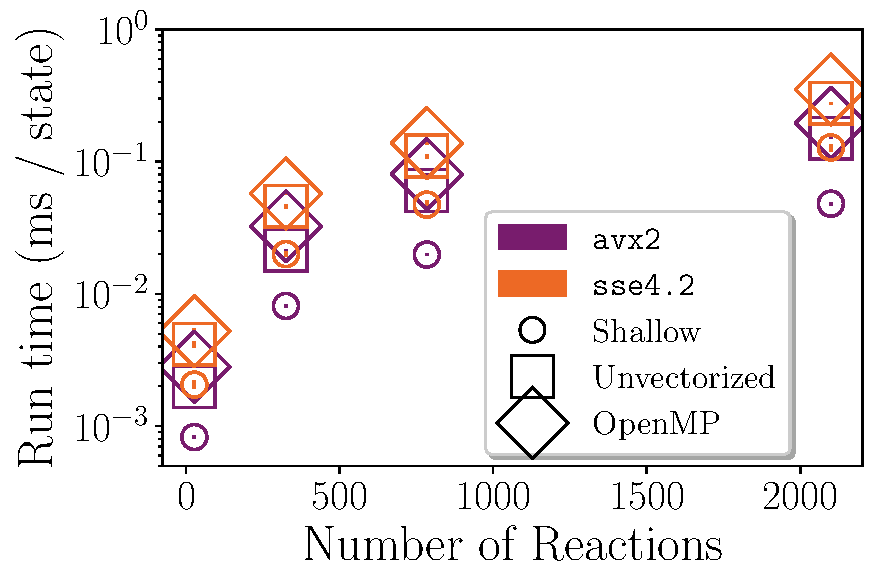
\includegraphics[width=\textwidth]{intel_source_nonorm.pdf}
      \caption{The mean run time per condition for each chemical model using the Intel OpenCL and OpenMP on both CPUs studied.}
      \label{F:intel_source_nonorm}
  \end{subfigure}
  \hfill
  \begin{subfigure}[t]{0.48\linewidth}
      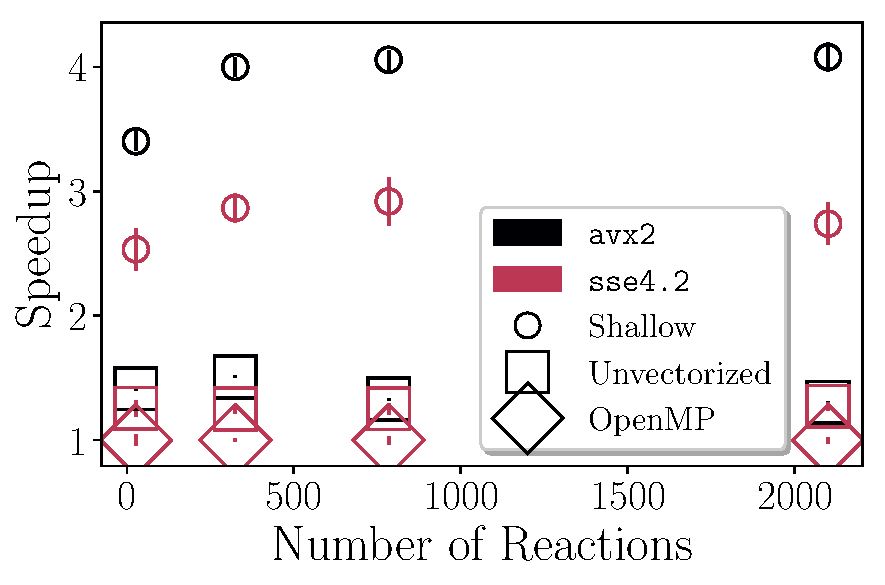
\includegraphics[width=\textwidth]{intel_source.pdf}
      \caption{The speedup achieved over the baseline OpenMP parallelization by both the unvectorized and shallow-vectorized Intel OpenCL codes; the speedup is presented on per-machine basis.}
      \label{F:intel_source}
  \end{subfigure}
  \\
  \begin{subfigure}[t]{0.48\linewidth}
      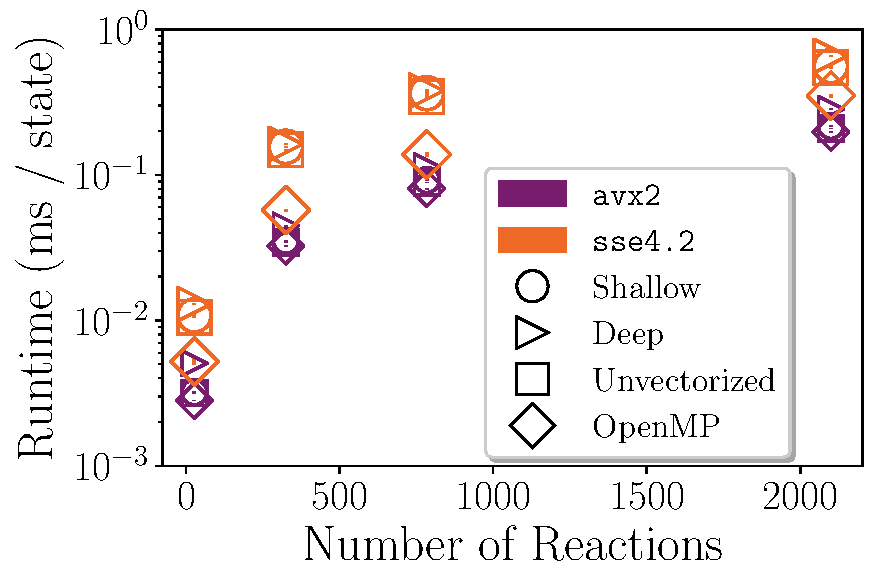
\includegraphics[width=\textwidth]{pocl_source_nonorm.pdf}
      \caption{The mean run time per condition of the Portable OpenCL runtime compared to OpenMP parallelization.}
      \label{F:pocl_source}
  \end{subfigure}
 \caption{Mean run times per condition and speedups achieved by the various CPU OpenCL runtimes compared to OpenMP parallelization for each chemical model studied. The names in the legends correspond to the identifiers listed in~\cref{t:cpus}.}
 \label{F:cpu_source}
\end{figure}

In~\cref{F:intel_source}, the extent of this speedup is detailed; we note that the speedup displayed is calculated per-machine, e.g., the \avx/ shallow-vectorized code speedup is relative to OpenMP on the same CPU such that the speedup of the shallow-vectorized OpenCL code can be readily assessed.
On both machines, the unvectorized OpenCL code is faster than the baseline parallel OpenMP code; by \SIrange{1.30}{1.51}{$\times$} on the \avx/ CPU, and \SIrange{1.25}{1.27}{$\times$} on the \sse/ machine.
Additionally, the shallow-vectorized OpenCL code is \SIrange{2.53}{2.92}{$\times$} and \SIrange{3.40}{4.08}{$\times$} faster than the OpenMP code for the \sse/ and \avx/ machines respectively.

In contrast,~\cref{F:pocl_source} shows the mean run time per condition of deep, shallow and unvectorized OpenCL codes on the POCL runtime, as compared to OpenMP parallelization.
No speedup is achieved for either vectorization type on either CPU; indeed the OpenMP case is faster on both CPUs.
The reasons for this lack of vectorization are quite technical and somewhat outside the scope of this work; however, briefly speaking vectorization might be achieved on POCL via a combination of fixed-array strides---rather than (potentially) varying with the number of initial conditions being evaluated, as currently is implemented---use of relaxed math (``\texttt{-cl-fast-relaxed-math}''), explicit OpenCL vector types and newer versions of LLVM\slash POCL (specifically, potential improvements to the vectorization module).
This will be explored more in future work, but for the moment POCL is still quite useful as a validation tool.

\Cref{F:gpu_source} shows the performance of the source-term evaluation on the GPUs listed in~\cref{t:gpus}.
In~\cref{F:gpu_source_scaling}, the number of initial conditions over which the source-terms are evaluated on the \gpunew/ GPU is varied in order to determine the effect on the mean run time per condition; the run time continues to decrease until \textasciitilde\num{e4} conditions for all chemical models (except the \ce{H2}\slash\ce{CO} model, which is closer to \textasciitilde\num{3e4} conditions), at which point the GPU becomes saturated and performance levels off.
\Cref{F:gpu_source_speedup} shows the speedup in source-term evaluations the \gpunew/ GPU over the \gpuold/ GPU for the maximum number of conditions in~\cref{F:gpu_source_scaling} for two different vector-widths (a.k.a., the block size in NVIDIA terminology), \num{64} and \num{128}; the fastest \gpunew/ case with a vector-width of 128 is \SIrange{1.40}{1.88}{$\times$} faster than the slowest case (\gpuold/ with a vector-width of \num{64}) depending on the chemical model in question.
Additionally,~\cref{F:gpu_source_speedup} shows that varying the vector-width has minimal effect on performance for most of the \gpunew/ and \gpuold/ cases; the GRI-Mech 3.0 and USC-Mech II models show the largest improvements with a vector-width of \num{128}, \textasciitilde\SIrange{10}{18}{\percent} for both GPUs.
This is likely caused by higher occupancy on the GPUs, however it is unclear exactly how NVIDIA's OpenCL runtime balances the registers\slash warps per streaming-multiprocessor, as controls occupancy in CUDA~\cite{occupancy}; use of even larger vector-widths (i.e., \num{256}\texttt{+}) on the GPU is a topic that merits future investigation.
\begin{figure}[htbp]
   \centering
  \begin{subfigure}[t]{0.48\linewidth}
      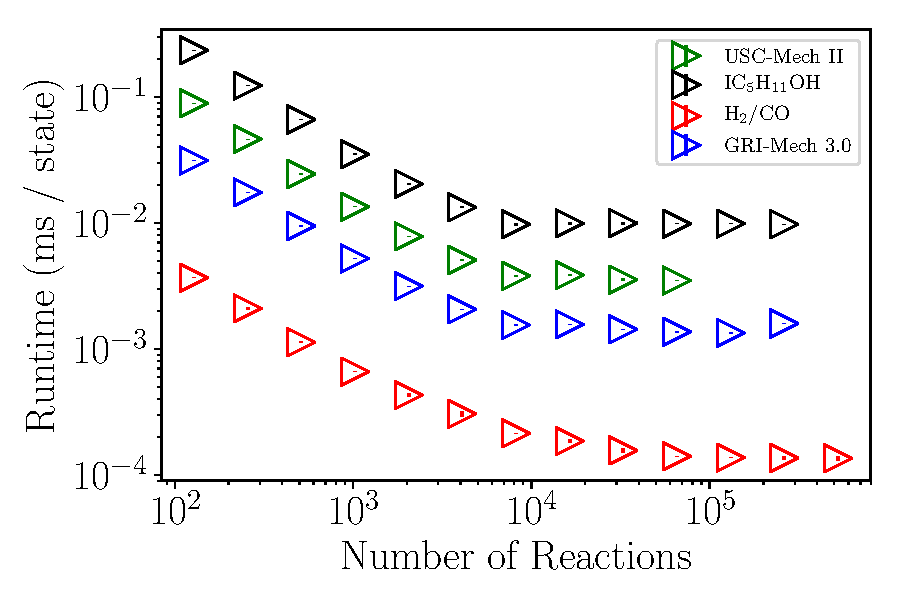
\includegraphics[width=\textwidth]{gpu_source_scaling.pdf}
      \caption{The mean run time per condition for each chemical model on the \gpunew/ GPU as a function of the number of initial conditions tested.}
      \label{F:gpu_source_scaling}
  \end{subfigure}
  \hfill
  \begin{subfigure}[t]{0.48\linewidth}
      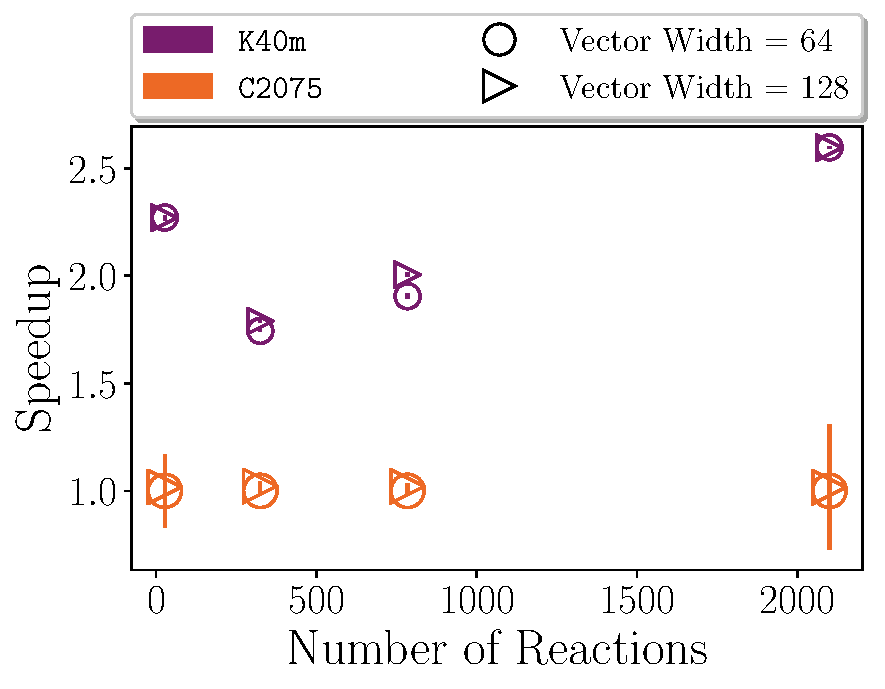
\includegraphics[width=\textwidth]{gpu_source_speedup.pdf}
      \caption{The speedup achieved on the \gpunew/ versus the \gpuold/ GPU; the names correspond to the identifiers listed in~\cref{t:gpus}}
      \label{F:gpu_source_speedup}
  \end{subfigure}
  \caption{\texttt{pyJac} source-term evaluation performance on the NVIDIA GPUs}
  \label{F:gpu_source}
\end{figure}

\Cref{f:source_permutate} shows the effect of changing data-ordering patterns, the \conp/ or \conv/ formulation, and the CPU vector-width size on the performance of source-term evaluation in \texttt{pyJac}.
In~\cref{F:source_conpvsconv}, it is seen that choice of the constant-pressure or constant-volume formulation has little to no effect on run time for OpenMP as well as the shallow-vectorized\slash unvectorized Intel OpenCL codes on the \avx/ machine.
Generally speaking, the difference between the \conp/ and \conv/ formulations has only a marginal effect on performance regardless of CPU\slash GPU choice.

\begin{figure}[htbp]
   \centering
  \begin{subfigure}[t]{0.48\linewidth}
      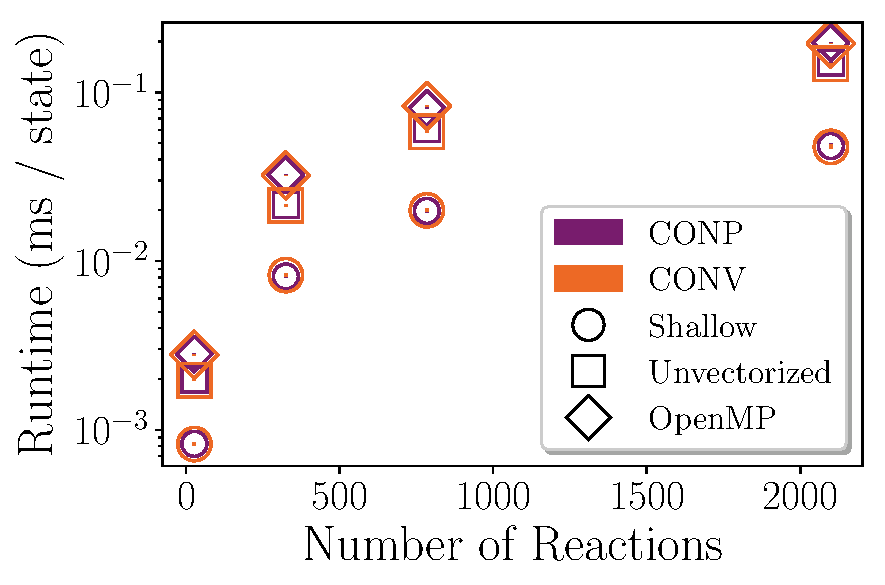
\includegraphics[width=\textwidth]{source_conpvsconv.pdf}
      \caption{The mean run time per condition for each chemical model using both the \conp/ and \conv/ formulations on Intel OpenCL and OpenMP on the \avx/ CPU.}
      \label{F:source_conpvsconv}
  \end{subfigure}
  \hfill
  \begin{subfigure}[t]{0.48\linewidth}
      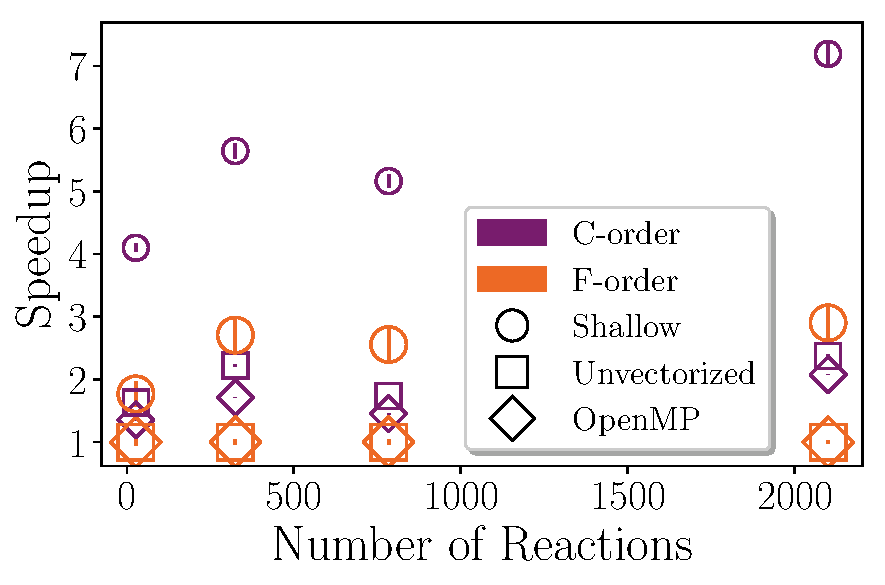
\includegraphics[width=\textwidth]{source_cvsf.pdf}
      \caption{The speedup achieved by ``C'' ordering over ``F'' ordering for Intel OpenCL and OpenMP on the \avx/ CPU.  The speedup presented is calculated per-language (OpenMP and OpenCL) to better assess the effect of the data-ordering.}
      \label{F:source_cvsf}
  \end{subfigure}
  \\
  \begin{subfigure}[t]{0.48\linewidth}
      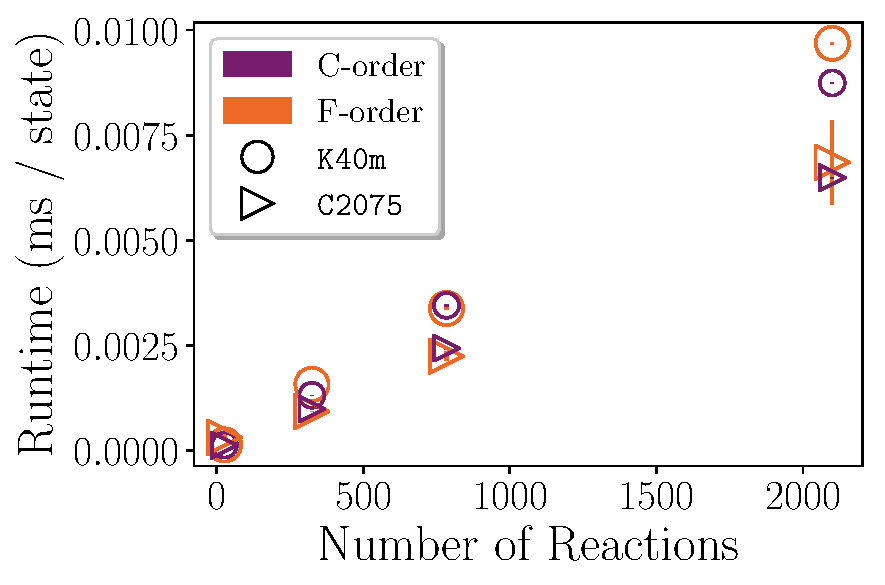
\includegraphics[width=\textwidth]{source_gpu_cvsf.pdf}
      \caption{The affect on performance of ``C'' vs ``F''-ordering for the shallow-vectorized NVIDIA OpenCL code on both GPUs with a vector-width of \num{128}.}
      \label{F:source_gpu_cvsf}
  \end{subfigure}
  \hfill
  \begin{subfigure}[t]{0.48\linewidth}
      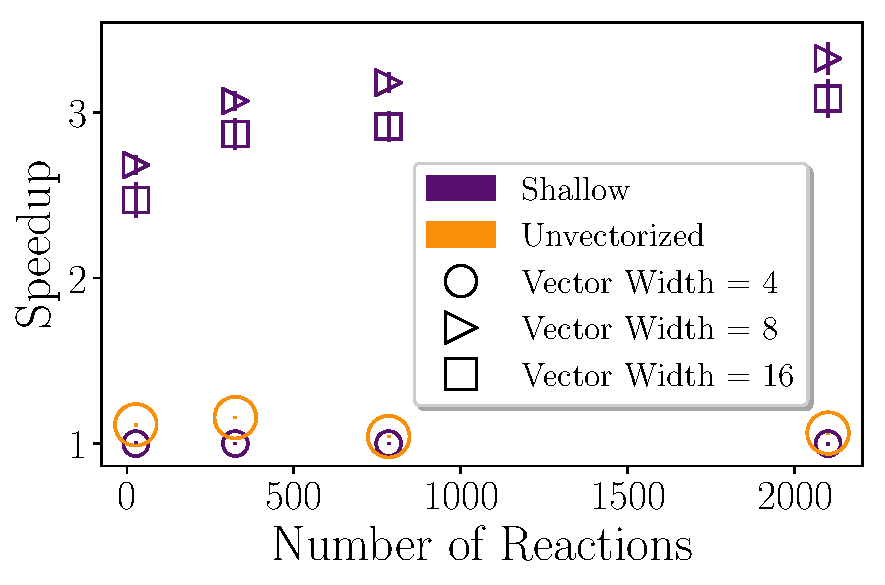
\includegraphics[width=\textwidth]{source_vector_width.pdf}
      \caption{The effect of vector-width on ``C''-ordered shallow-vectorized Intel OpenCL source-term evaluations in the \avx/ CPU.}
      \label{F:source_vector_width}
  \end{subfigure}
  \caption{The effect of the \conp/ and \conv/ formulations, ``C'' and ``F'' data-ordering, and CPU vector-width on source-term evaluation performance in \texttt{pyJac}.
	   It is noted the shallow-vectorized ``C'' ordered OpenCL cases corresponds to the vectorized data ordering described in~\cref{S:data}}
  \label{f:source_permutate}
\end{figure}

In contrast,~\Cref{F:source_cvsf} shows significant speedups of ``C''-ordered data over ``F''-ordered data on the \avx/ machine; the speedup presented is calculated per language, e.g., the \SIrange{1.35}{2.09}{$\times$} speedup of the ``C''-ordered OpenMP implementation is relative to the ``F''-ordered OpenMP baseline.
Additionally, it is noted that the ``C''-ordered shallow-vectorization in~\cref{F:source_cvsf} utilizes the vectorized-data ordering described in~\cref{S:data}; this case achieves speedups of \SIrange{2.14}{2.58}{$\times$} over the ``F''-ordered shallow-vectorization, demonstrating the value of the vectorized data ordering for CPU execution.

\Cref{F:source_gpu_cvsf} shows the performance effect of the ``C'' versus ``F''-ordering on source-term evaluation performance on both GPUs, with the speedup presented per-GPU.
In general, the ``C'' and ``F''-ordered shallow-vectorizations are nearly equivalent on both GPUs, with less than a \SI{10}{\percent} difference in run time between data-orderings. 
It is noted that for the isopentanol model, ``C''-ordered data is \textasciitilde\SI{1.08}{$\times$} faster on both GPUs (while the trend is less clear for the other models).
The rough equivalence between the ``C'' and ``F''-ordered codes GPUs is counter to what one might expect, as typically speaking coalesced memory access in a shallow-vectorization is easier to achieve if ``F''-ordering is used (see~\cref{S:data}).
However, the vectorized-data ordering here ensures that not only are memory accesses aligned to the vector-width size and thus, likely well-coalesced.

\Cref{F:source_vector_width} shows the effect of changing vector-width size on source-term performance the \avx/ CPU.
The vector-width of size \num{8} was the fastest tested, while the larger vector-width of \num{16} is slightly slower due to increased register pressure~\cite{intel_vectypes}.
It is unclear why the vector-width of \num{4} results in no speedup at all (it is in fact, the slowest case); Intel's vectorization guide~\cite{intel_vecknobs} mentions that a heuristic determines the optimal vector-width (in this case, it appears from compiler output to be \num{8}), so it is possible using vector-width smaller than the heuristic breaks the implicit vectorizer.
It is noted that this issue does not occur for a vector-width of \num{4} on the \sse/ CPU.


Finally,~\cref{F:source_scaling} displays the (strong) parallel scaling efficiency and SIMD efficiency for the CPU platforms.
The strong parallel scaling efficiency is defined as:
\begin{equation}
 \label{e:strong_scaling}
 \varepsilon = \frac{\bar{t}_{1}}{N \bar{t}_{N}}
\end{equation}
where $\bar{t}_{N}$ is the mean run time per condition on $N$ CPU cores, and $\bar{t}_{1}$ the same on a single CPU core.
The strong parallel scaling efficiency measures the speedup due to the use of additional CPU cores, as a fraction of linear speedup; strong scaling tends to decrease with the number of processors used due to memory bandwidth limitations and decreasing computation work allocated per CPU core~\cite{strong_scaling}.

\begin{figure}[htbp]
   \centering
  \begin{subfigure}[t]{0.48\linewidth}
      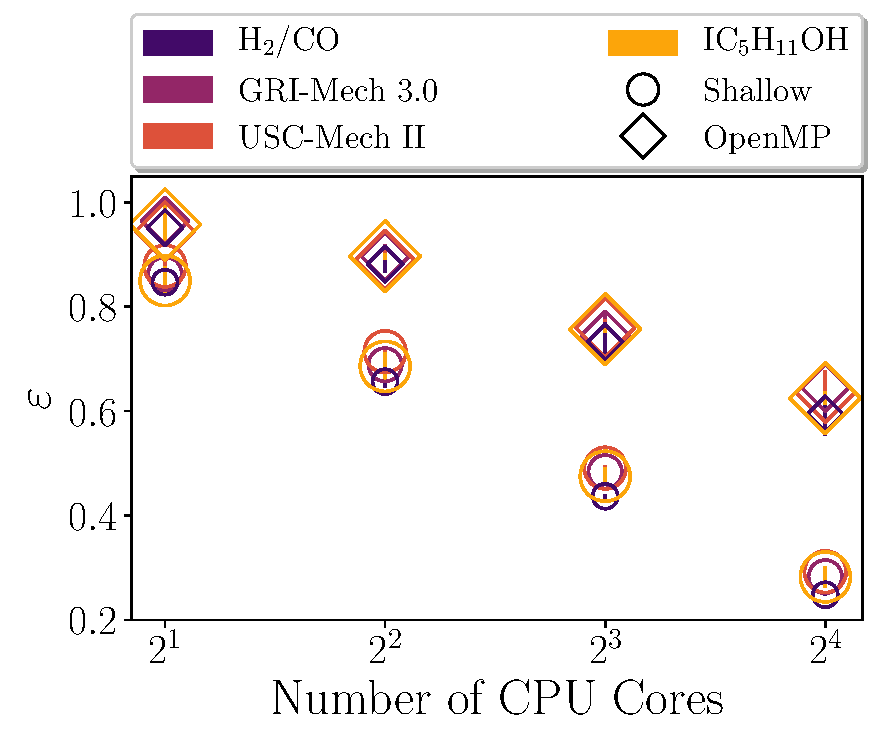
\includegraphics[width=\textwidth]{source_parallel_scaling.pdf}
      \caption{The strong parallel scaling efficiency (as defined in~\cref{e:strong_scaling}) of source-term evaluation for Intel OpenCL\slash OpenMP on the \avx/ machine.}
      \label{F:source_parallel_scaling}
  \end{subfigure}
  \hfill
  \begin{subfigure}[t]{0.48\linewidth}
      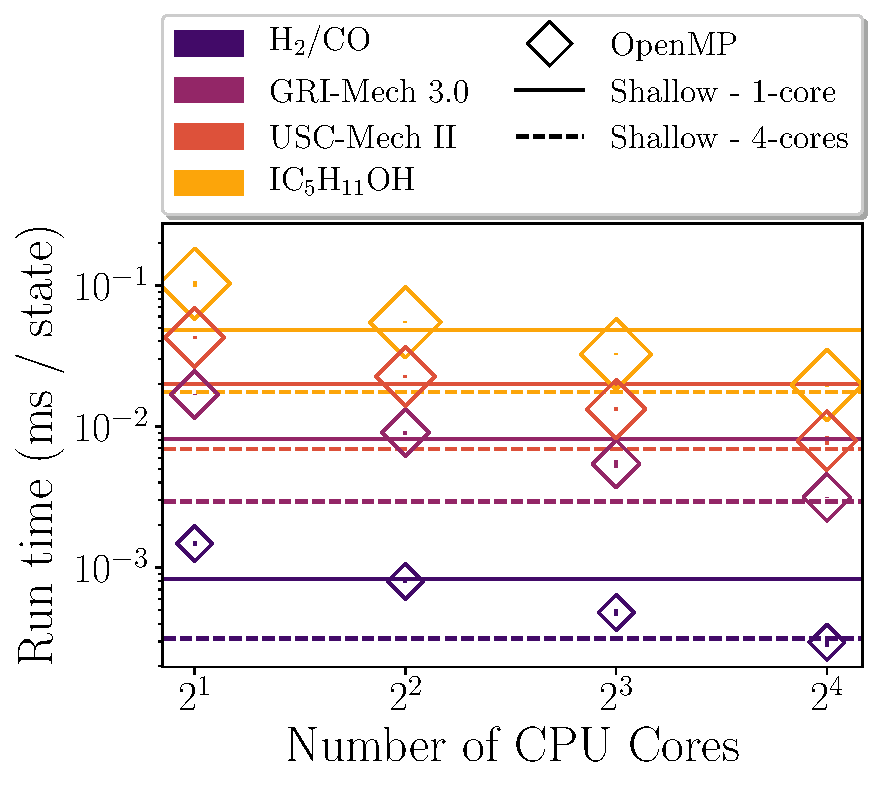
\includegraphics[width=\textwidth]{source_crossover.pdf}
      \caption{The mean run time per-condition of OpenMP source-term evaluation on different cores compared to a shallow-vectorized Intel OpenCL evaluation on \num{1} (solid lines) and \num{4} (dashed lines) cores on \avx/ machine.}
      \label{F:source_crossover}
  \end{subfigure}
  \\
  \begin{subfigure}[t]{0.48\linewidth}
      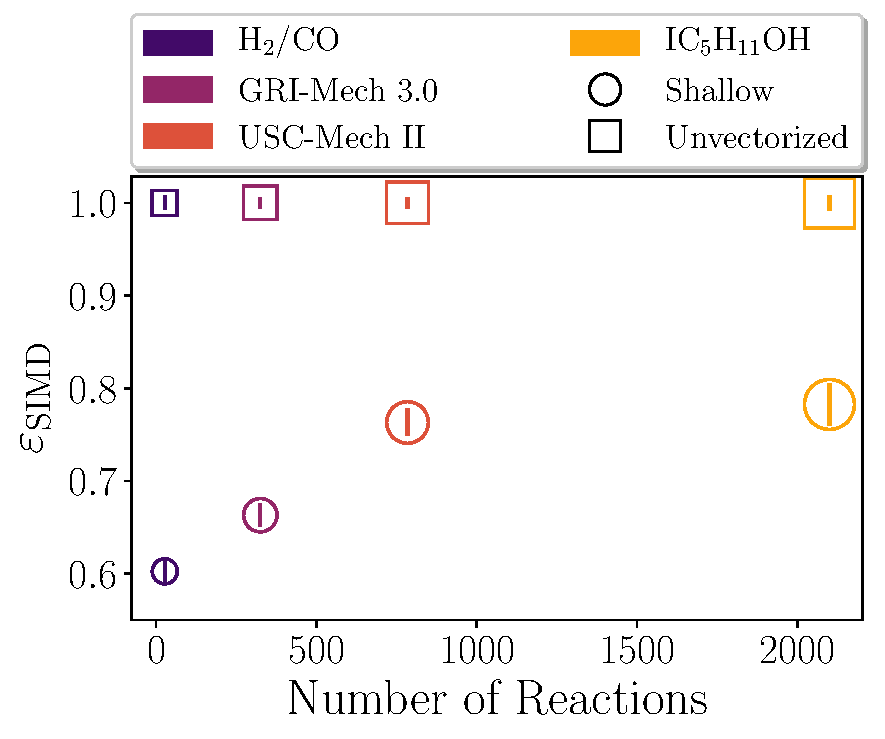
\includegraphics[width=\textwidth]{source_simd_efficiency.pdf}
      \caption{The SIMD efficiency (\cref{e:simd_efficiency}) of source-term evaluation for the Intel OpenCL runtime on a single core of the \avx/ CPU.}
      \label{F:source_simd_scaling}
  \end{subfigure}
  \hfill
  \begin{subfigure}[t]{0.48\linewidth}
      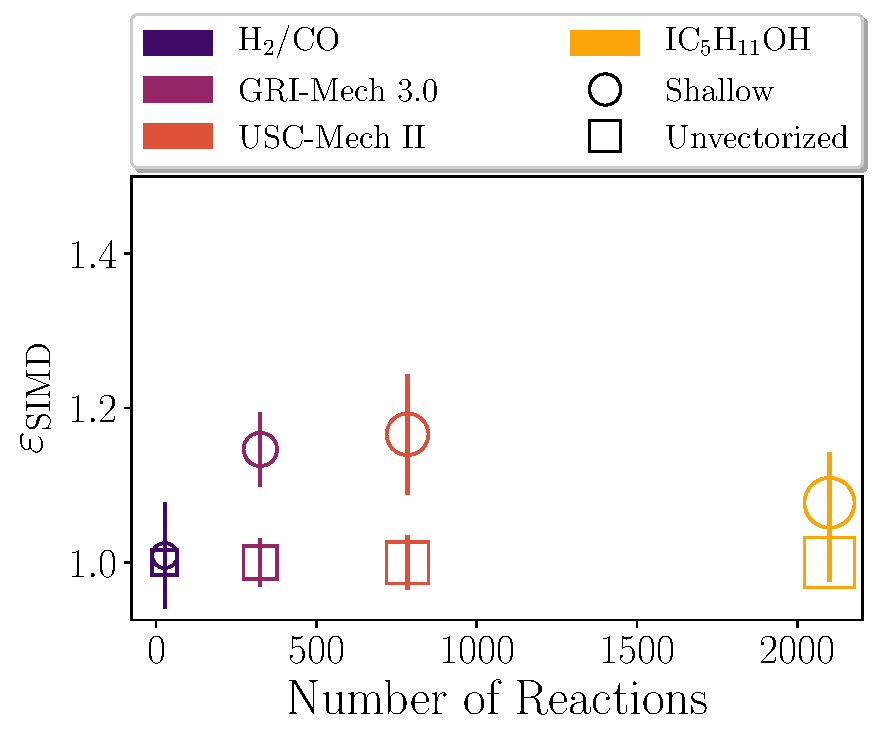
\includegraphics[width=\textwidth]{source_sse_simd_efficiency.pdf}
      \caption{The SIMD efficiency (\cref{e:simd_efficiency}) of source-term evaluation for the Intel OpenCL runtime on a single core of the \sse/ CPU.}
      \label{F:source_sse_simd_scaling}
  \end{subfigure}
  \caption{The parallel scaling efficiency and SIMD efficiency of source-term evaluation for Intel OpenCL on the \avx/ and \sse/ CPUs.}
  \label{F:source_scaling}
\end{figure}

\Cref{F:source_parallel_scaling} shows the strong parallel scaling efficiency of source-term evaluation in \texttt{pyJac} on the \avx/ machine for both the shallow-vectorized Intel OpenCL and OpenMP codes.
In general, the \ce{H2}\slash\ce{CO} mechanism has the worst scaling efficiency for Intel OpenCL; although the mechanism scalings vary somewhat for OpenMP, there is no clear trend.
It is likely the poor scaling of the \ce{H2}\slash\ce{CO} for Intel OpenCL results from both its relatively small size, and few falloff\slash chemically activated reaction (in particular, the additional expensive logarithm and exponential evaluations that accompany them); i.e., there is simply not enough work to fully utilize the SIMD instructions.
Additionally, OpenMP tends to have higher scalings then the shallow-vectorized OpenCL code, e.g., \textasciitilde\num{0.9} and \textasciitilde\num{0.75} for \num{4} and \num{8} CPU cores respectively, compared to just \numrange{0.66}{0.72} and \numrange{0.44}{0.48} for OpenCL; although not pictured (to keep the figure readable), the unvectorized Intel OpenCL code has only slightly worse scaling than the OpenMP code, hence the poorer scaling is unique to the shallow-vectorizated code.
This is due in large part to the superior performance of the shallow-vectorized OpenCL code, coupled with the relatively small amounts of work associated with source-term evaluation.
To illustrate this,~\cref{F:source_crossover} shows the mean run time per-condition of the OpenMP source-term evaluations for \numrange{2}{16} cores, compared to the shallow-vectorized OpenCL code on \num{1} (solid line) and \num{4} (dashed line) four cores on the \avx/ machine.
For all chemical models, the mean run time per-condition (and hence the computational work allocated per-core, one of the key-drivers of parallel scaling efficiency~\cite{strong_scaling}) of OpenMP running on \num{4} cores is roughly equal to that of the shallow-vectorized OpenCL code on a single core.
Similarly, OpenMP running on \num{16} cores is roughly equivalent to the OpenCL code on \num{4} cores.
Therefore, a more fair comparison of parallel scaling efficiencies is to compare OpenCL running on \num{4} cores, to OpenMP on \num{16}; the OpenMP code's parallel efficiency drops to \textasciitilde\num{0.64} for \num{16} cores, similar to OpenCL's parallel scaling efficiency of \numrange{0.66}{0.72} at \num{4} cores.
Indeed, as will be investigated in~\cref{S:jacobian_results} the strong parallel scaling efficiency for sparse Jacobian evaluation---the most computationally intensive task in this work---are far more similar between Intel OpenCL and OpenMP.

The SIMD efficiency is defined as:
\begin{equation}
 \label{e:simd_efficiency}
 \varepsilon_{\text{SIMD}} = \frac{\bar{t}_{\text{unvec}}}{W \bar{t}_{\text{shallow}}}
\end{equation}
where $\bar{t}_{\text{unvec}}$ is the mean run time per condition of the unvectorized OpenCL code, $\bar{t}_{\text{shallow}}$ the same for the shallow-vectorized OpenCL code, and $W$, the vector-width reported in number of double operations in~\cref{t:cpus}.
This measure compares the actual speedup due to shallow-vectorization compared to the nominal vector-width of the machine in question.
\Cref{F:source_simd_scaling} shows the SIMD efficiency of source-term evaluation in \texttt{pyJac} on a single core of the \avx/ machine; the larger models (isopentanol and USC-Mech II) have higher SIMD-efficiency of \numrange{0.76}{0.78}, and the smaller models (\ce{H2}\slash\ce{CO}, GRI-Mech \num{3.0}) have lower SIMD-efficiency, \numrange{0.6}{0.66}.
This again demonstrates that the SIMD-vectorization becomes efficient as the amount of work to perform increases (with increasing model size).
Interestingly,~\cref{F:source_sse_simd_scaling} shows the SIMD efficiency on the \sse/ machine as greater than one; this is likely caused by a combination of use of an OpenCL vector-width greater than the native CPU vector-width (i.e., \num{8} v.s., \num{2}), and the improved data-locality for the vectorized-data ordering, as discussed in~\cref{S:data}, and results a modest \SIrange{7}{17}{\percent} improvement over the nominal vector-width.


\subsubsection{Jacobian evaluation}
\label{S:jacobian_results}

\begin{figure}[htbp]
   \centering
  \begin{subfigure}[t]{0.48\linewidth}
      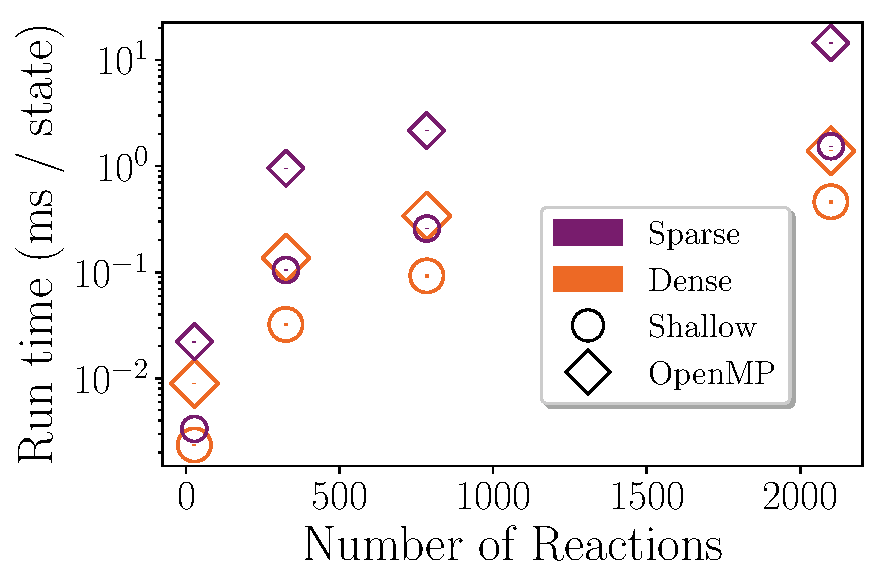
\includegraphics[width=\textwidth]{sparse_vs_dense.pdf}
      \caption{The mean run time per-condition of sparse and dense Jacobian evaluation for Intel OpenCL\slash OpenMP on the \avx/ machine.}
      \label{F:sparse_vs_dense}
  \end{subfigure}
  \hfill
  \begin{subfigure}[t]{0.48\linewidth}
      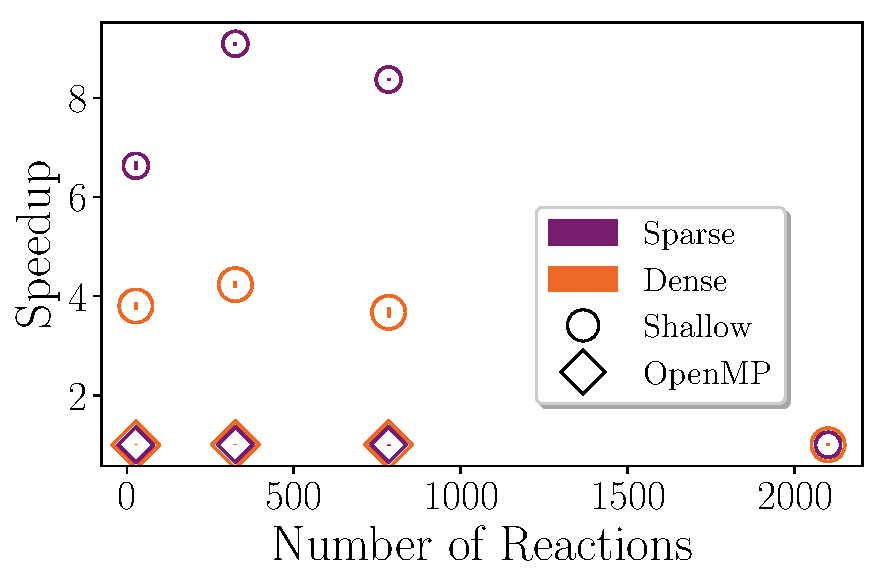
\includegraphics[width=\textwidth]{sparse_vs_dense_speedup.pdf}
      \caption{The speedup of the sparse and dense Jacobian evaluation for Intel OpenCL over the sparse\slash dense OpenMP baseline on the \avx/ machine.}
      \label{F:sparse_vs_dense_speedup}
  \end{subfigure}
  \\
  \begin{subfigure}[t]{0.48\linewidth}
      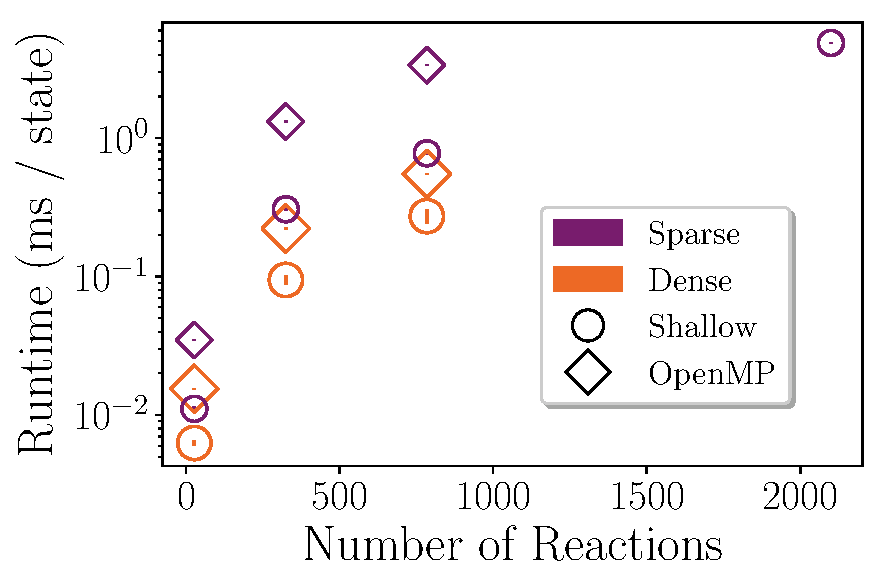
\includegraphics[width=\textwidth]{sparse_vs_dense_sse.pdf}
      \caption{The mean run time per-condition of sparse and dense Jacobian evaluation for Intel OpenCL\slash OpenMP on the \sse/ machine.}
      \label{F:sparse_vs_dense_sse}
  \end{subfigure}
  \hfill
  \begin{subfigure}[t]{0.48\linewidth}
      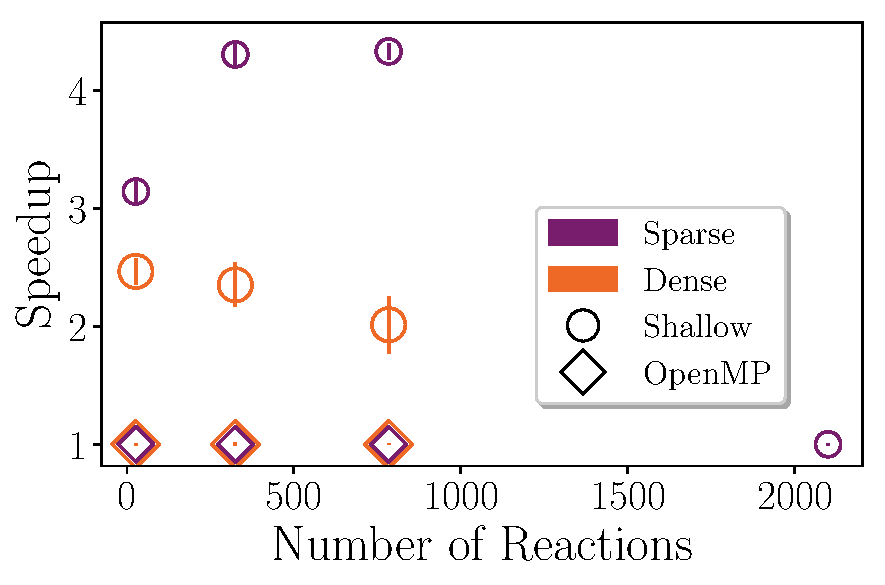
\includegraphics[width=\textwidth]{sparse_vs_dense_see_speedup.pdf}
      \caption{The speedup of the sparse and dense Jacobian evaluation for Intel OpenCL over the sparse\slash dense OpenMP baseline on the \sse/ machine.}
      \label{F:sparse_vs_dense_sse_speedup}
  \end{subfigure}
  \caption{Performance of sparse and dense Jacobian evaluation on the CPU platforms in \texttt{pyJac}.}
  \label{F:jacobian_perfomance}
\end{figure}

\Cref{F:jacobian_perfomance} shows the performance of the sparse and dense Jacobian evaluations in \texttt{pyJac} on the CPU platforms.
In~\cref{F:sparse_vs_dense}, the mean run time per condition is presented for the shallow-vectorized Intel OpenCL and OpenMP codes on the \avx/ CPU.
The sparse Jacobian evaluations are slower on both Intel OpenCL and OpenMP due to indirect lookup indexing requirements, as discussed in~\cref{S:sparsity}.
Interestingly the shallow-vectorized OpenCL code is less negatively impacted by the indirect lookup; the sparse OpenMP code is \SIrange{2.47}{10.42}{$\times$} slower than the dense OpenMP evaluation, while the sparse shallow-vectorized OpenCL code is just \SIrange{1.41}{3.34}{$\times$} slower than its dense counterpart
As a result, the shallow-vectorized sparse OpenCL code is as fast, or faster than the dense OpenMP code in all cases on the \avx/ machine (\cref{F:sparse_vs_dense}).
\Cref{F:sparse_vs_dense_speedup} shows the speedup of the sparse\slash dense shallow-vectorized OpenCL the over the same sparse\slash dense Jacobian format on OpenMP; the dense OpenCL code is \SIrange{3.03}{4.23}{$\times$} faster than the corresponding dense OpenMP code, this speedup increases to \SIrange{6.63}{9.44}{$\times$} for the sparse Jacobian.

On the \sse/ machine,~\cref{F:sparse_vs_dense_sse} shows similar results; the sparse OpenMP code is the slowest in all cases, and the shallow-vectorized OpenCL code is nearly as fast as the dense OpenMP code.
Once again, the sparse OpenCL code is far less negatively impacted by the indirect lookup, and is only \SIrange{1.76}{3.33}{$\times$} slower than its dense counterpart, while the sparse OpenMP code is significantly (\SIrange{2.25}{8.72}{$\times$}) slower than the dense version.
In~\cref{F:sparse_vs_dense_sse_speedup}, the speedup of the sparse and dense shallow-vectorized OpenCL codes are compared to their OpenMP version; the dense OpenCL code is \SIrange{1.92}{2.47}{$\times$} faster, while the sparse shallow-vectorization achieves a speedup of \SIrange{3.14}{5.03}{$\times$}.

\begin{figure}[htbp]
   \centering
  \begin{subfigure}[t]{0.48\linewidth}
      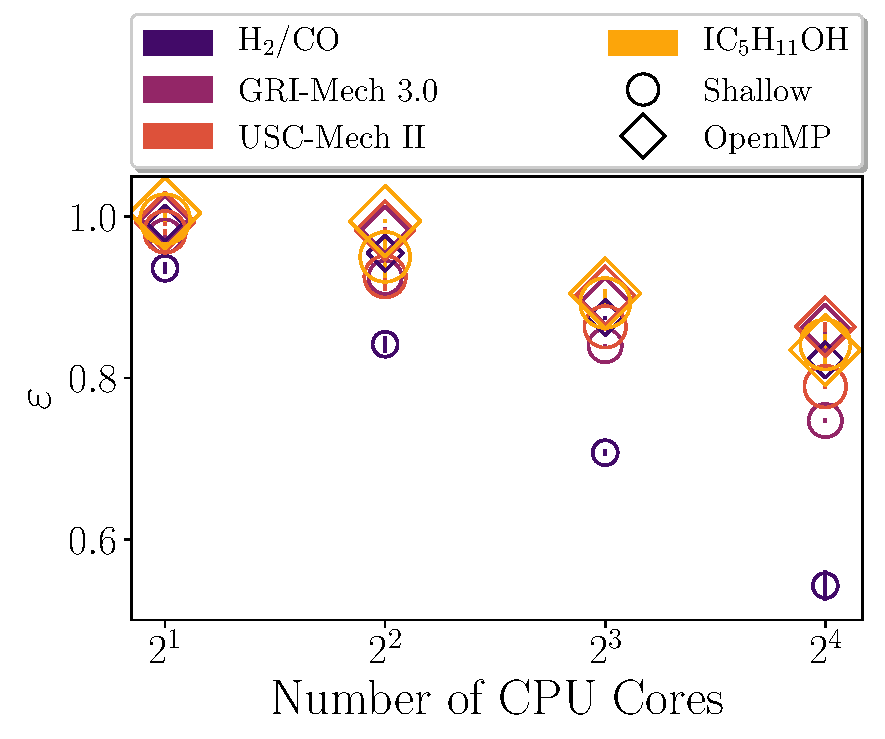
\includegraphics[width=\textwidth]{sparse_jac_scaling.pdf}
      \caption{Sparse Jacobian evaluation parallel scaling efficiency for Intel OpenCL\slash OpenMP on the \avx/ machine.}
      \label{F:sparse_jac_scaling}
  \end{subfigure}
  \hfill
  \begin{subfigure}[t]{0.48\linewidth}
      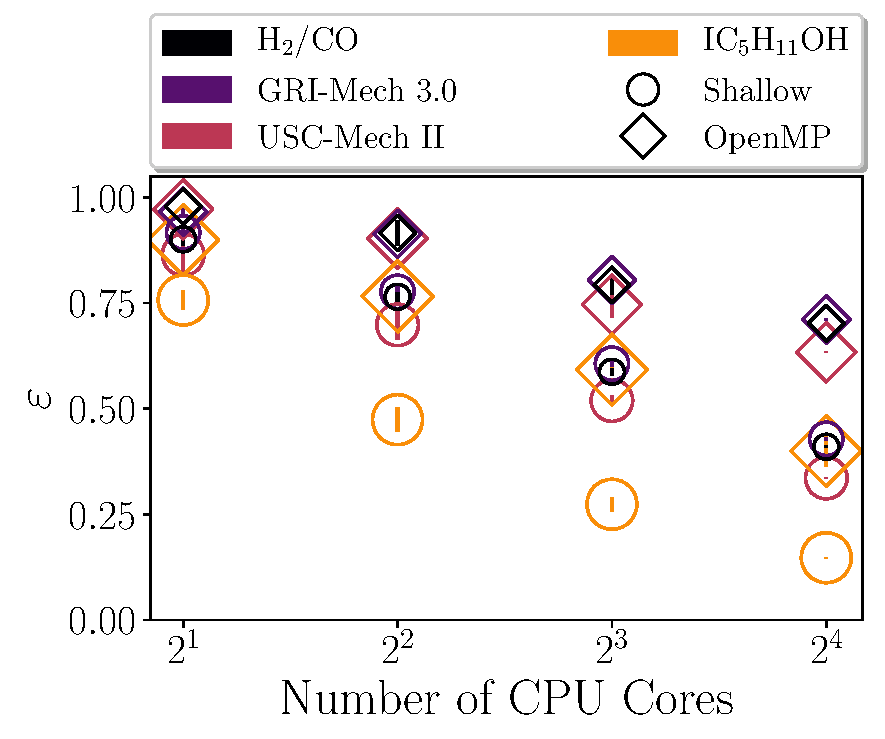
\includegraphics[width=\textwidth]{dense_jac_scaling.pdf}
      \caption{Dense Jacobian evaluation parallel scaling efficiency for Intel OpenCL\slash OpenMP on the \avx/ machine.}
      \label{F:dense_jac_scaling}
  \end{subfigure}
  \caption{The parallel scaling efficiencies of sparse and dense Jacobian evaluation for the shallow-vectorized Intel OpenCL and OpenMP codes on the \avx/ CPU.}
\end{figure}

In~\cref{F:sparse_jac_scaling}, the strong parallel scaling efficiency of the sparse shallow-vectorized OpenCL is compared to the sparse OpenMP code.
The plot is a bit difficult to read, as most of the data-points are clustered together, however the key takeaway is that the parallel scaling efficiency of the shallow-vectorized OpenCL code is very similar to that of the OpenMP code, in contrast to the source-terms parallel scaling efficiencies (\cref{F:source_parallel_scaling}).
The \ce{H2}\slash\ce{CO} model has the worst scaling for both codes, ranging from \numrange{0.94}{0.54} and \numrange{0.99}{0.82} for OpenCL and OpenMP respectively on \numrange{2}{16} cores.
As the model size increases, the efficiency of the OpenCL code improves dramatically, reaching \numrange{0.997}{0.84} for the isopentanol model.
\Cref{F:dense_jac_scaling} shows scaling for the shallow-vectorized dense Jacobian OpenCL code.
In this case, the isopentanol model has the worst scaling for both codes, it is noted that due to the sheer size of the dense isopentanol Jacobian---storing the dense matrix for a single thermo-chemical state takes over \SI{1}{\mega\byte} of data---the total number of states for the dense isopentanol Jacobian evaluation was limited to \num{50000} (which requires over \SI{50}{\giga\byte} of memory); this greatly drops the computation cost for this case, and adversely affects the scaling efficiency as was discussed in~\cref{S:source_results}.
Excluding the isopentanol model, the dense shallow-vectorized OpenCL scalings are slightly higher than for source-term evaluation, e.g., \numrange{0.70}{0.78} and \numrange{0.52}{0.61} for \num{4} and \num{8} cores respectively (compared to \numrange{0.66}{0.72} and \numrange{0.44}{0.48} for shallow-vectorized OpenCL source-term on the same \num{4} and \num{8} cores); this is due to the higher computational cost of Jacobian evaluation, and hence more available work per CPU-core.
As in~\cref{S:source_results}, we note that the shallow-vectorized dense Jacobian code running on \num{1} and \num{4} cores of the \avx/ machine is roughly as fast as the OpenMP code on \num{4} and \num{16} cores respectively; the parallel scaling efficiency of OpenMP at \num{16} cores (excluding isopentanol as previously) is \numrange{0.63}{0.71}, similar to the shallow-vectorization's efficiency of \numrange{0.70}{0.78} for \num{4} cores.

\begin{figure}[htbp]
   \centering
  \begin{subfigure}[t]{0.48\linewidth}
      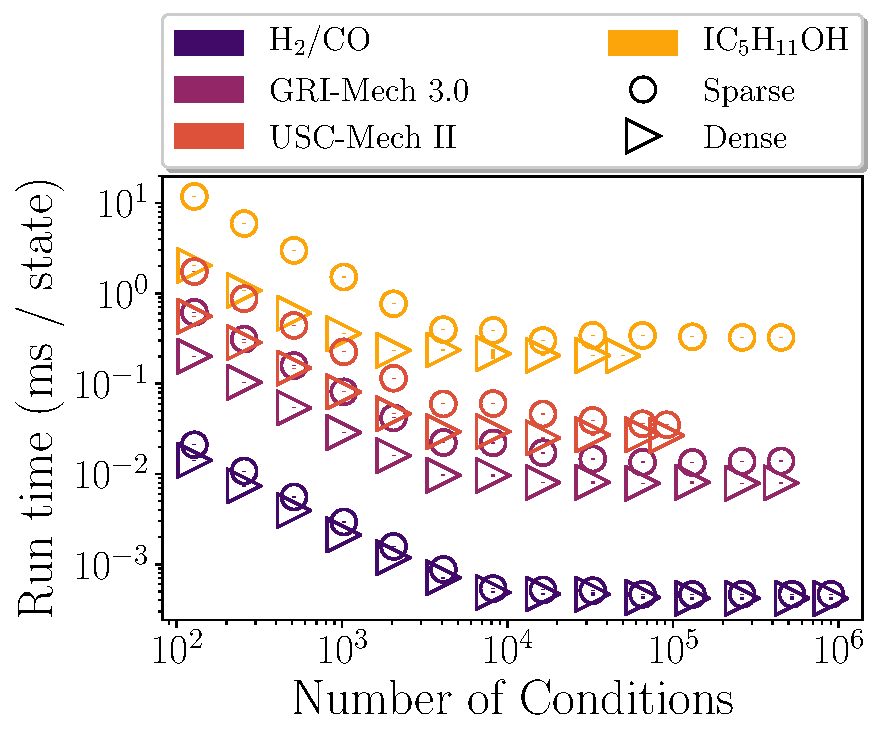
\includegraphics[width=\textwidth]{gpu_sparse_vs_dense.pdf}
      \caption{Mean run time per-condition of sparse and dense Jacobian evaluation on the \gpunew/ GPU.}
      \label{F:gpu_sparse_vs_dense}
  \end{subfigure}
  \hfill
  \begin{subfigure}[t]{0.48\linewidth}
      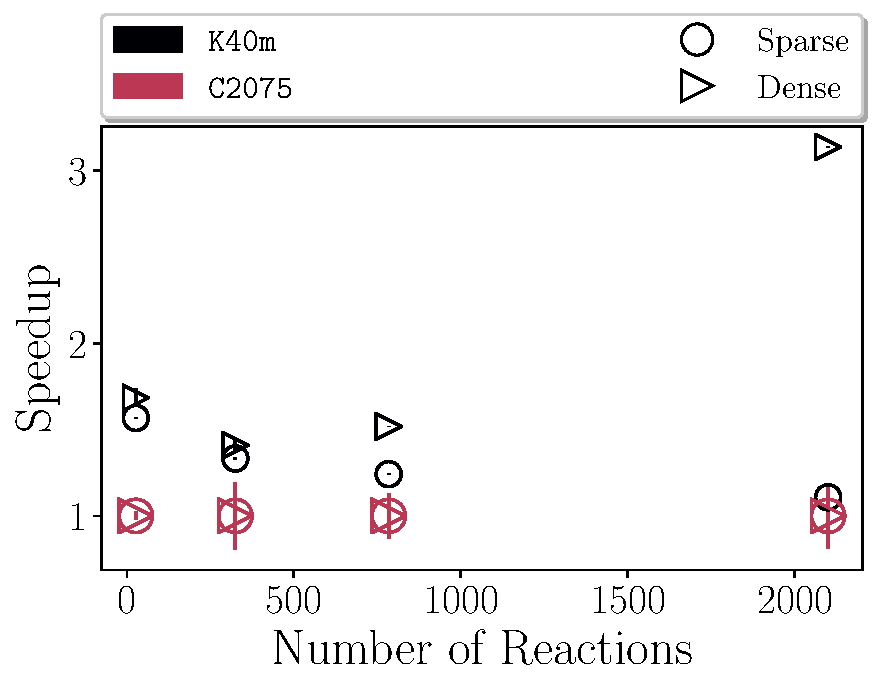
\includegraphics[width=\textwidth]{gpu_jacobian_speedup.pdf}
      \caption{Speedup of the \gpunew/ over \gpuold/ GPUs for sparse and dense Jacobian evaluation, normalized per-Jacobian type (i.e., sparse versus dense).}
      \label{F:gpu_jacobian_speedup}
  \end{subfigure}
  \caption{The performance of sparse\slash dense Jacobian evaluation on the \gpunew/ and \gpuold/ GPUs.}
\end{figure}

The mean run time per-condition for the sparse and dense Jacobian evaluation on the \gpunew/ GPU is plotted in~\cref{F:gpu_sparse_vs_dense}.
As in the species evaluation case, the mean run time per-condition drops steadily, for both cases becoming roughly constant after just \num{3e3} states (except for \ce{H2}\slash\ce{CO}, which levels off near \num{e4} conditions).
Sparse Jacobian evaluation is significantly slower for all models before the GPU becomes saturated (due to the indirect indexing lookup), however past the saturation point the performance gap between the sparse and dense evaluations narrows.
This is likely caused by the combination of being able to fit many more sparse Jacobian matrices in the \gpunew/'s memory, as well as improved data-locality\slash caching due to the smaller size of the sparse Jacobian.
\Cref{F:gpu_jacobian_speedup} presents the speedup of the \gpunew/ over the \gpuold/ GPU for sparse\slash dense Jacobian evaluation; sparse evaluation on the \gpunew/ is \SIrange{1.10}{1.59}{$\times$} faster than on the \gpuold/, while dense evaluation is \SIrange{1.36}{3.0}{$\times$} faster.
The speedup on the \gpunew/ appears to decrease with increasing mechanism size for the sparse evaluation, but increases for the larger models in dense evaluation; this is likely due to the larger memory size of the \gpunew/, and hence fewer data-transfer operations.


In~\cref{F:fd_vs_analytical}, the performance of the sparse analytical-Jacobian is compared to a sparse first-order finite-difference Jacobian on both the \avx/ CPU and the \gpuold/ \gpunew/ GPUs.
\Cref{F:fd_vs_analytical_cpu} shows large speedups for both the OpenMP code and shallow-vectorized OpenCL code; the analytical OpenMP Jacobian is \SIrange{3.92}{8.67}{$\times$} faster, while the analytical OpenCL Jacobian achieves speedups of \SIrange{17.22}{55.11}{$\times$}.
It is noted that the isopentanol case was excluded here, as a single run of the sparse finite-difference Jacobian using either OpenCL or OpenMP took over \num{12} hours of run time.
In addition the current finite-difference formulation breaks Intel's auto-vectorizer, hence the OpenCL speedup comparison is made against the unvectorized OpenCL code; it is not a high priority to fix this issue, as the finite-difference Jacobian is implemented for comparison purposes only.
Although we do not display the dense finite-difference Jacobian speedup in~\cref{F:fd_vs_analytical_cpu}, the dense OpenCL and OpenMP analytical Jacobian codes out-perform the finite-difference variants by even larger margins; \SIrange{24.44}{245.63}{$\times$} for OpenCL, and \SIrange{9.68}{112.73}{$\times$} for OpenMP (these data do include the isopentanol model, though limited to \num{50000} conditions as discussed previously).
A comparison of the sparse analytical and finite-difference Jacobians on the GPUs is presented in~\cref{F:fd_vs_analytical_gpu}.
The analytical Jacobian on the \gpunew/ and \gpuold/ shows large speedups, increasing with chemical model size, in the range of \SIrange{3.81}{17.60}{$\times$}; the \gpunew/ has a larger speedup than the \gpuold/ (\SI{17.60}{$\times$} v.s., \SI{14.75}{$\times$}) for the isopentanol model due to it's larger memory size.
Although not pictured, the dense analytical-Jacobian on the \gpunew/ GPU has larger speedups compared with the dense finite-difference Jacobian: \SIrange{4.04}{45.13}{$\times$}; the \gpunew/ GPU again has a significantly larger speedup than the \gpuold/ for the isopentanol model (\SI{45.13}{$\times$} vs \SI{23.85}{$\times$}), further underscoring the effect of the larger available memory on the \gpunew/.

\begin{figure}[htbp]
   \centering
  \begin{subfigure}[t]{0.48\linewidth}
      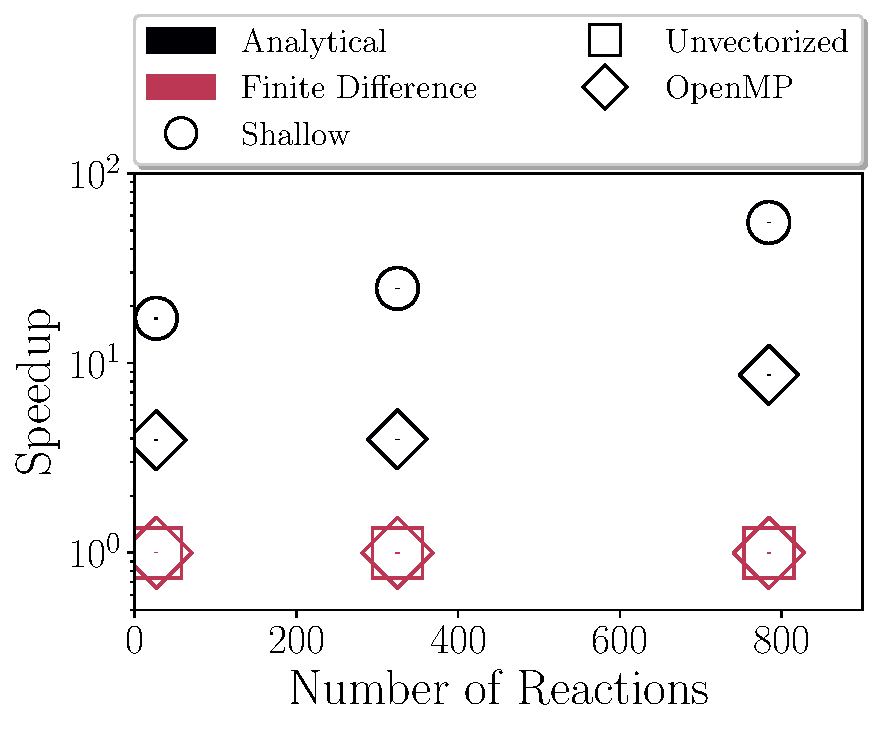
\includegraphics[width=\textwidth]{finite_difference_vs_analytical.pdf}
      \caption{Speedup of the sparse analytical Jacobian versus finite-difference Jacobian evaluation on the \avx/ CPU, normalized per-language}
      \label{F:fd_vs_analytical_cpu}
  \end{subfigure}
  \hfill
  \begin{subfigure}[t]{0.48\linewidth}
      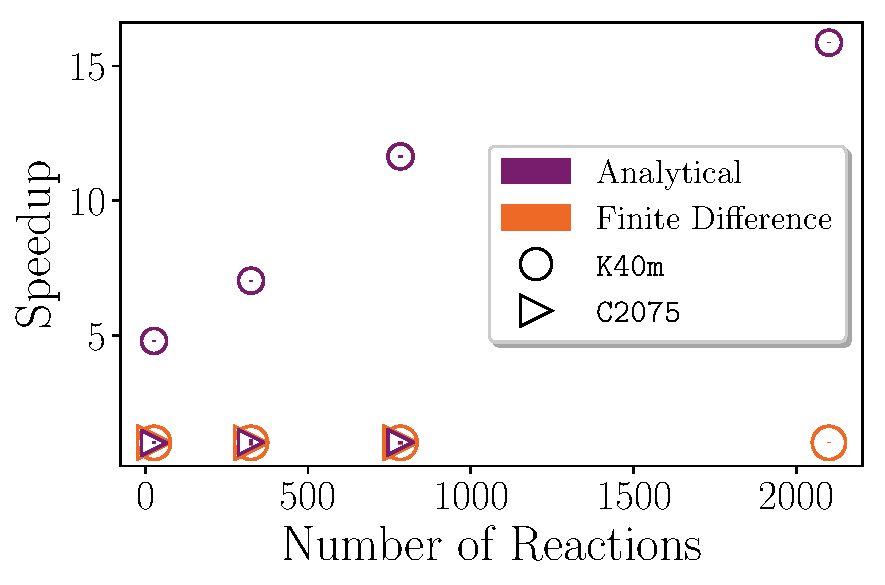
\includegraphics[width=\textwidth]{finite_difference_vs_analytical_gpu.pdf}
      \caption{Speedup of the analytical versus finite-difference Jacobian evaluation on both the \gpunew/ and \gpuold/ GPUs, normalized per-GPU}
      \label{F:fd_vs_analytical_gpu}
  \end{subfigure}
  \caption{The performance of a sparse, first-order forward finite-difference Jacobian compared to the analytical Jacobian on the \avx/ CPU and both GPUs.}
  \label{F:fd_vs_analytical}
\end{figure}

\Cref{F:v1_vs_v2} compares the performance for evaluation of the dense-analytical Jacobian of the new version of \texttt{pyJac} to the previous version~\cite{pyjac16} on the \sse/ CPU and \gpuold/ GPU; dense Jacobian evaluation was selected as it was the only type implemented in the previous version of \texttt{pyJac}.
On the \sse/ CPU, the \texttt{pyJac-v2} is faster than \texttt{pyJac-v1} for OpenMP evaluation for the larger chemical models; the static OpenMP code generated by \texttt{pyJac-v1} (see~\cref{s:unittest}) is \SI{1.79}{$\times$} faster for the \ce{H2}\slash\ce{CO} model, and only \SI{1.09}{$\times$} slower for the GRI-Mech 3.0 model.
In contrast, the loop-based OpenMP code of \texttt{pyJac-v2} is \SIrange{3.37}{10.19}{$\times$} faster than \texttt{pyJac-v1} for the USC-Mech II and isopentanol models.
The shallow-vectorized OpenCL code is faster than \texttt{pyJac-v1} in all cases, achieving speedups of \SIrange{1.37}{19.56}{$\times$} increasing with model size.
In~\cref{F:v1_vs_v2_gpu}, the performance of the \texttt{pyJac-v2} dense-analytical Jacobian on the \gpuold/ GPU is compared to \texttt{pyJac-v1} on the same.
As with the CPU, the static code of \texttt{pyJac-v1} is slightly faster for the \ce{H2}\slash\ce{CO} model, however \texttt{pyJac-v2} outperforms \texttt{pyJac-v1} by \SIrange{1.25}{2.84}{$\times$} for the other models; it is noted that the decrease in speedup for the isopentanol model is likely due to the limited number of conditions in dense-evaluation for \texttt{pyJac-v2}, as noted earlier.

\begin{figure}[htbp]
   \centering
  \begin{subfigure}[t]{0.48\linewidth}
      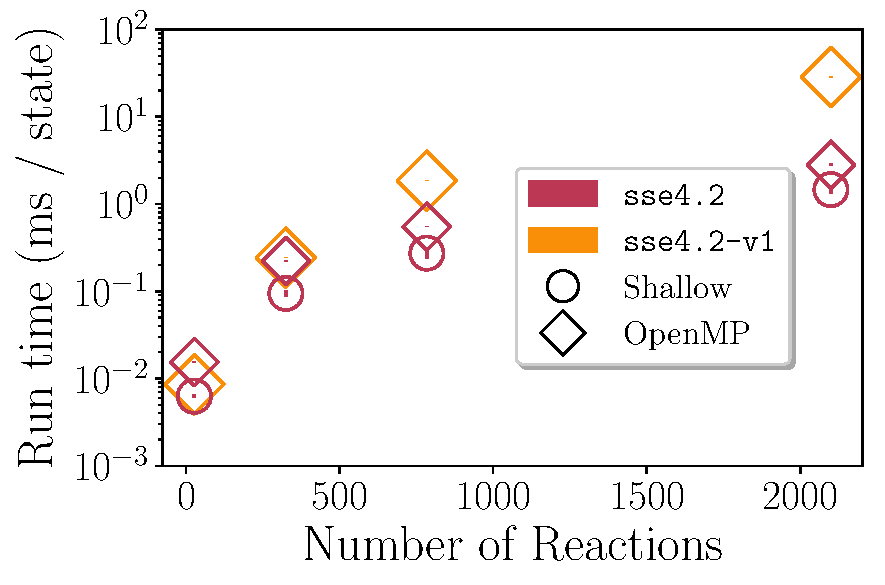
\includegraphics[width=\textwidth]{v1_vs_v2.pdf}
      \caption{Speedup of dense Jacobian evaluation in \texttt{pyJac-v2} over \texttt{pyJac-v1} on the \sse/ CPU}
      \label{F:v1_vs_v2_cpu}
  \end{subfigure}
  \hfill
  \begin{subfigure}[t]{0.48\linewidth}
      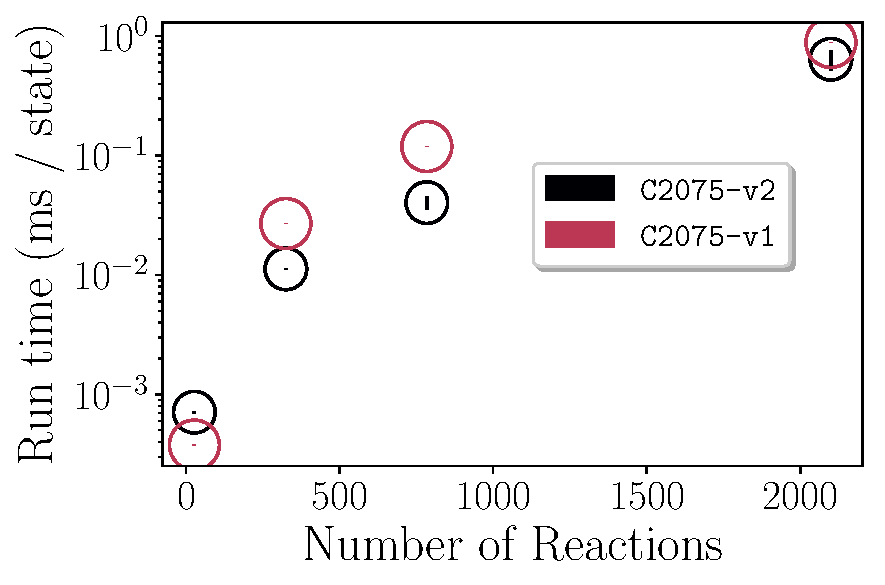
\includegraphics[width=\textwidth]{v1_vs_v2_gpu.pdf}
      \caption{Speedup of dense Jacobian evaluation in \texttt{pyJac-v2} over \texttt{pyJac-v1} on the \gpuold/ GPU}
      \label{F:v1_vs_v2_gpu}
  \end{subfigure}
  \caption{Performance comparison of the new version of \texttt{pyJac} (\texttt{v2}) and the previous version, \texttt{v1}~\cite{pyjac16}.}
  \label{F:v1_vs_v2}
\end{figure}



\section{Future directions and practical notes on OpenCL usage}
\label{s:future}
It is important to note that while OpenCL provides an easy way to enable cross-platform execution, and significant speedups were achieved via shallow-vectorized OpenCL code in this work, there are some serious potential pit-falls in its use.
Typically speaking, the closed source OpenCL runtimes tested in this work (Intel and NVIDIA) contain bugs that result in compilation failures, simply incorrect vectorized machine code or even segmentation faults; further, these runtimes (in our experience) tend to be less responsive to fixing said bugs, with relatively infrequent new releases (or in NVIDIA's case, changelogs\slash public records of bug-fixes).
On the other hand, the open-source OpenCL runtime used in this work, POCL, has (in our experience) far fewer implementation bugs, and when issues arise the community is very responsive to bug reports and user outreach; however, POCL fails to achieve vectorization as noted in~\cref{S:source_results}.

As demonstration of the type of issue we're discussing, a minimum working example has been created~\cite{nvidia_mwe} that demonstrates a failure of NVIDIA's OpenCL runtime corresponding to the GPU driver version \num{375.26} on a Tesla K40m GPU; by simply changing to another runtime (e.g., Intel), with no other code changes, the correct result can be found.
This provides a particularly vexing problem for the programmer, as there is often little that can be done to resolve the issue; thankfully, in this case we were able to upgrade the driver version to resolve the problem.
Further, as noted throughout this work certain transformations or code-generation patterns can break OpenCL execution\slash vectorization; e.g., the failure of POCL to achieve vectorization or Intel OpenCL's failure to vectorize the finite-difference Jacobian.
Indeed the vectorization attempted by the OpenCL runtimes (or reasons for incorrectly vectorized code) are not always obvious to the user.
It is possible, particularly for the Intel OpenCL \slash POCL runtimes, that better performance might be achieved using so called ``explicit'' vectorization, i.e., through use of built-in vector types such as the \texttt{double8}.
This will be investigated in future works.

Thankfully, \texttt{loo.py} allows relatively easy switching between output languages; the most significant code change is building the wrapper that initializes\slash transfers memory and calls the kernel.
Indeed, the OpenMP code-generation built into \texttt{pyJac} is currently only capable of parallel-execution, but extending this platform to shallow\slash deep-vectorizations (via \texttt{loo.py} and compiler pragmas) is a key priority going forwards.
In addition, CUDA~\cite{NVIDIA:2018} and Intel's open-source OpenCL alternative ISPC~\cite{pharr2012ispc} have been significantly more reliable in previous works~\cite{Niemeyer:2016aa,CurtisGPU:2017} and (in the case of ISPC) initial testing.
The current deep-vectorization formulation would be executable for both CUDA and ISPC targets, as these languages implement double-precision atomic operations, further recommending their use.
Extending execution to these targets to make CPU\slash GPU more reliable vectorization is a future goal.


\section{Conclusions}
In this work, automatically generated OpenCL codes for shallow SIMD-vectorized thermo-chemical source-term evaluation were developed and validated against Cantera~\cite{Cantera} for a shallow range of chemical kinetic models~\cite{Burke:2011fh,smith_gri-mech_30,Wang:2007,Sarathy:2013jr}.
Significant speedups of up to \SIrange{1.90}{2.45}{$\times$} over a baseline SIMT-vectorized code were observed.
Two data-ordering schemes were investigated, showing a clear performance benefit for use of the ``C'' (row-major) ordering for the shallow vectorized code.
Further, this study suggests that a deep SIMD-vectorized code---currently under development---may see even greater accelerations due to expected increases in cache-hit rates.
Larger vector-widths were found to provide accelerations for the smaller models studied, but the speedup was similar over all vector-widths tested for the largest models investigated.
Finally, the strong parallel scaling efficiency was examined for the shallow vectorized code; the larger models exhibited higher scaling efficiency, possibly due to failure of the \ce{H2}\slash\ce{CO} model to saturate the CPU throughput.
Future extensions of this work will include development of a SIMD\slash SIMT-accelerated sparse-analytical Jacobian code targeted at CPUs, GPUs, and MICs.

\section{Acknowledgments}
This research was funded by the National Science Foundation under grant ACI-1534688.

\bibliography{paper}

\end{document}
